% =====================================================================
%  Machine Learning for Biological Age -- A Research Roadmap
%  Companion to Bioage_Machine_Learning.ipynb
%  Build:  latexmk -pdf Bioage_Research_Roadmap.tex   (or pdflatex twice)
% =====================================================================
\documentclass[11pt,a4paper]{article}

% ---- Edit these three lines before circulating -----------------------
\newcommand{\preparedby}{Enrique Zuazua (FAU Erlangen-N\"urnberg)}
\newcommand{\docversion}{Version 1.0}
\newcommand{\docdate}{29 September 2026}
% ----------------------------------------------------------------------

\usepackage[T1]{fontenc}
\usepackage[utf8]{inputenc}
\usepackage{lmodern}
\usepackage{microtype}
\usepackage[margin=2.3cm,headheight=14pt]{geometry}
\usepackage{amsmath,amssymb,amsthm,mathtools}
\usepackage{graphicx}
\usepackage{booktabs,tabularx,array,longtable}
\usepackage[table]{xcolor}
\usepackage{enumitem}
\usepackage{xparse}
\usepackage{caption}
\usepackage{fancyhdr}
\usepackage{titlesec}
\usepackage[most]{tcolorbox}
\usepackage[colorlinks=true,linkcolor=navy,citecolor=teal,urlcolor=teal]{hyperref}
\usepackage[capitalise,noabbrev]{cleveref}
\crefname{problem}{Problem}{Problems}
\newcommand{\card}[1]{\hyperref[card:#1]{project~#1}}
\setlength{\emergencystretch}{2.5em}

\graphicspath{{figures/}}

% ---- Palette (matches the notebook) ---------------------------------
\definecolor{navy}{HTML}{183B56}
\definecolor{teal}{HTML}{16877C}
\definecolor{ochre}{HTML}{9A6A12}
\definecolor{plum}{HTML}{5B4A8B}
\definecolor{rust}{HTML}{B04A36}
\definecolor{forest}{HTML}{2D6A4F}
\definecolor{slate}{HTML}{6B7C86}

\titleformat{\section}{\Large\bfseries\color{navy}}{\thesection}{0.8em}{}
\titleformat{\subsection}{\large\bfseries\color{navy}}{\thesubsection}{0.7em}{}
\titleformat{\subsubsection}{\normalsize\bfseries\color{teal}}{\thesubsubsection}{0.6em}{}

\pagestyle{fancy}
\fancyhf{}
\fancyhead[L]{\small\color{slate}ML for biological age: a research roadmap}
\fancyhead[R]{\small\color{slate}\docversion\ $\cdot$ \docdate}
\fancyfoot[C]{\small\thepage}
\renewcommand{\headrulewidth}{0.3pt}

\setlist{itemsep=2pt,topsep=4pt}
\setlength{\parskip}{3pt}
\renewcommand{\arraystretch}{1.18}
\captionsetup{font=small,labelfont={bf,color=navy}}

% ---- Callout boxes ---------------------------------------------------
\newtcolorbox{callout}[2]{enhanced,breakable,colback=#1!6!white,colframe=#1,
  boxrule=0pt,leftrule=4pt,arc=2pt,left=8pt,right=8pt,top=5pt,bottom=5pt,
  fonttitle=\bfseries\small,coltitle=#1,colbacktitle=#1!6!white,
  title={\MakeUppercase{#2}},attach title to upper={\par\smallskip}}
\newenvironment{opportunity}{\begin{callout}{ochre}{Opportunity}}{\end{callout}}
\newenvironment{conclusion}{\begin{callout}{teal}{Main conclusion}}{\end{callout}}
\newenvironment{scope}{\begin{callout}{rust}{Scope}}{\end{callout}}
\newenvironment{perspective}{\begin{callout}{forest}{Perspective}}{\end{callout}}
\newenvironment{translation}{\begin{callout}{plum}{Translation}}{\end{callout}}

\newtcolorbox{projectcard}[2]{enhanced,breakable,colback=white,colframe=navy,
  boxrule=0.6pt,arc=2pt,left=8pt,right=8pt,top=4pt,bottom=4pt,
  fonttitle=\bfseries,colbacktitle=navy,coltitle=white,title={#1\quad #2}}
\newcommand{\field}[1]{\par\noindent\textbf{\color{navy}#1.}\ }

% ---- Theorems --------------------------------------------------------
\theoremstyle{plain}
\newtheorem{theorem}{Theorem}[section]
\newtheorem{proposition}[theorem]{Proposition}
\newtheorem{corollary}[theorem]{Corollary}
\newtheorem{lemma}[theorem]{Lemma}
\theoremstyle{definition}
\newtheorem{definition}[theorem]{Definition}
\newtheorem{example}[theorem]{Example}
\newtheorem{problem}{Problem}
\renewcommand{\theproblem}{\arabic{problem}}
\theoremstyle{remark}
\newtheorem{remark}[theorem]{Remark}

% ---- Evidence labels -------------------------------------------------
\newcommand{\tagbox}[2]{\tcbox[on line,boxsep=1pt,left=2pt,right=2pt,top=0pt,bottom=0pt,
  colback=#1!12!white,colframe=#1,boxrule=0.4pt,arc=1pt]{\scriptsize\bfseries\color{#1}#2}}
\newcommand{\REP}{\tagbox{teal}{REPORTED}}
\newcommand{\PROP}{\tagbox{ochre}{PROPOSAL}}
\newcommand{\NEW}{\tagbox{plum}{NEW HERE}}
\NewDocumentCommand{\PI}{o}{\textup{[P1\IfValueT{#1}{, #1}]}}
\NewDocumentCommand{\PII}{o}{\textup{[P2\IfValueT{#1}{, #1}]}}

% ---- Maths macros ----------------------------------------------------
\newcommand{\E}{\mathbb{E}}
\newcommand{\R}{\mathbb{R}}
\newcommand{\Var}{\operatorname{Var}}
\newcommand{\Cov}{\operatorname{Cov}}
\newcommand{\corr}{\operatorname{corr}}
\DeclareMathOperator*{\argmin}{argmin}

\begin{document}

% =====================================================================
\begin{titlepage}\sloppy
\begin{tcolorbox}[colback=navy,colframe=navy,arc=4pt,left=18pt,right=18pt,top=18pt,bottom=18pt]
\color{white}
{\small\color{teal!40!white}\bfseries BIOLOGY $\times$ MATHEMATICS $\cdot$ RESEARCH ROADMAP}\par\medskip
{\LARGE\bfseries Machine Learning for Biological Age}\par\smallskip
{\Large From an interpretable NMR clock and a rigidity theorem\\ to the next generation of joint projects}\par\bigskip
{\normalsize Working document for the MetAge--SHAP collaboration\\
CIC bioGUNE $\cdot$ ATLAS Molecular Pharma $\cdot$ CIBERehd $\cdot$ FAU Erlangen-N\"urnberg $\cdot$ DeustoTech--University of Deusto $\cdot$ Universidad Aut\'onoma de Madrid}
\end{tcolorbox}

\vspace{1.2em}
\noindent\textbf{Prepared by:} \preparedby\\
\textbf{Status:} \docversion, \docdate. Internal working document.\\
\textbf{Companion material:} the teaching notebook \texttt{Bioage\_Machine\_Learning.ipynb}, its HTML editions, and the code in the same folder.

\vspace{1.2em}
\noindent\textbf{Built on two manuscripts of the collaboration}
\begin{description}[leftmargin=2.4em,style=nextline]
\item[\PI] A.~Ib\'a\~nez de Opakua, M.~Bizkarguenaga, \dots, U.~Biccari, R.~Morales, \dots, E.~Zuazua, J.~M.~Mato, \'O.~Millet (multi-centre consortium).
\emph{Mapping metabolic aging and disease-associated acceleration using an interpretable NMR-based clock.} Manuscript \texttt{MetAgePaper\_submitted.pdf}.
\item[\PII] U.~Biccari, A.~Ib\'a\~nez de Opakua, J.~M.~Mato, \'O.~Millet, R.~Morales, E.~Zuazua.
\emph{Fair feature attribution for multi-output prediction: a Shapley-based perspective.} Manuscript \texttt{SHAP\_SIMODS\_03.pdf}.
\end{description}
Page, figure, table and theorem numbers refer to these manuscript versions. Both may still change before publication, so please do not circulate this document outside the collaboration without the authors' consent.

\vspace{1.2em}
\begin{tcolorbox}[colback=white,colframe=slate,boxrule=0.4pt,arc=2pt,title={\small\bfseries How to read this document},colbacktitle=slate!10!white,coltitle=navy]
\small
\textbf{Purpose.} This document hands the collaboration a common starting point: what the two papers established, a shared mathematical language, the open problems, and concrete project and paper proposals, so that each of us can take up a thread.

\textbf{Evidence labels.} \REP\ is a result quoted from \PI\ or \PII, not recomputed here. \NEW\ is a mathematical statement proved in this document or in the notebook. It is not a claim of either paper. \PROP\ marks a research design, conjecture or project idea.

\textbf{Two audiences.} Boxes marked \textsc{Translation} restate mathematical content for biologists and biological content for mathematicians. \cref{app:glossary} is a two-way glossary.
\end{tcolorbox}
\end{titlepage}

\tableofcontents
\newpage

% =====================================================================
\section{Executive summary}
\label{sec:summary}

\begin{opportunity}
A single serum NMR measurement can be turned into an \textbf{interpretable map} of how metabolism ages and of how each disease distorts that path \PI. Rigorous \textbf{multi-output explanation} makes one shared model explainable output by output, with a theorem behind the practice \PII. Making these maps reliable, transportable, dynamic and linked to the genome is a research programme that needs geneticists and mathematicians working together.
\end{opportunity}

\paragraph{What is established.}
\begin{enumerate}
\item \REP\ \emph{A unified interpretable clock} \PI. A curated set of 75 NMR-derived variables predicts chronological age over 7--106 years with $r=0.88$ and RMSE $8.7$\,y. Its condition number is $\kappa\approx16$, against $\kappa\approx15{,}000$ for spectral bins, which are more accurate ($r=0.93$, RMSE $6.5$\,y). One model serves both sexes. On an independent Austrian laboratory it reaches $r=0.81$, although the RMSE rises to $12.2$\,y.
\item \REP\ \emph{A coherent biological signature} \PI. Inflammation and immune activity is the leading SHAP group (16.9\% of the grouped magnitude). Albumin and erythrocyte sedimentation rate (ESR) are the leading individual features.
\item \REP\ \emph{Disease maps} \PI. All eleven disease cohorts (3,882 patients) are shifted toward older metabolic profiles, from $2.8$\,y (long COVID) to $17.5$\,y (influenza), while the negative controls are not. The shifts separate along renal, inflammatory and strictly metabolic axes. Individuals who later had a cardiovascular event were already about $8$\,y older metabolically. IBD in remission shows about $3$\,y less distortion than active disease.
\item \REP\ \emph{Rigidity theorem} \PII. Under the classical Shapley axioms imposed verbatim for vector-valued games, attribution for $f:\R^n\to\R^m$ must be coordinate-wise. Any rule that couples outputs violates at least one axiom. The vector operator is Lipschitz-stable in the game and in the predictor.
\item \REP\ \emph{Joint learning in practice} \PII. On 15,931 observations (outputs: age, MetSCORE, sex), one shared network trained $2.79\times$ faster than three separate ones. It matched them on MetSCORE and sex and gave aligned explanations (cosine similarity $\ge0.974$), although it was slightly less accurate for age.
\end{enumerate}

\paragraph{What this document adds.}
\NEW\ A unified notation (\cref{sec:framework}). Two short results that sharpen the interpretation of age gaps: the slope of the optimal clock equals $R^2$ (\cref{prop:gap}), and a unit-slope clock pays a factor $1/r$ in RMSE (\cref{prop:duality}). A ledger separating established from open claims (\cref{sec:ledger}). Sixteen precisely stated research problems (\cref{sec:math,sec:bio}). Seven joint project cards (\cref{sec:joint}), a paper pipeline (\cref{sec:papers}) and a first-year plan (\cref{sec:plan}).

\paragraph{Five flagship proposals} \PROP
\begin{description}[leftmargin=1.2em,font=\color{navy}]
\item[J1 \,Multi-axis clock.] Renal, inflammatory and hepatic-metabolic ages as outputs of one shared model. The rigidity theorem makes the per-output explanations rigorous (\card{J1}).
\item[J2 \,Trait or state?] Longitudinal distortion dynamics, and a \emph{dynamic SHAP} theory that links explainability to control (\card{J2}).
\item[J3 \,Transportable clocks.] Multi-laboratory harmonisation, shift-aware conformal uncertainty and equivalence testing (\card{J3}).
\item[J4 \,Certified explanations.] From the empirical agreement of Table~4 of \PII\ to data-driven stability certificates (\card{J4}).
\item[J5 \,From metabolic age to the genome.] Genetic architecture of metabolic distortion (clock-GWAS, Mendelian randomisation) under explicit assumptions (\card{J5}).
\end{description}

% =====================================================================
\section{The problem and its challenges}
\label{sec:problem}

Two people aged 60 can differ in physiological reserve, inflammatory burden, renal function and disease risk. ``Biological age'' names this heterogeneity, but no ground-truth label for it is ever observed. Serum metabolites are end products and intermediates of metabolic pathways: they integrate genetic background, long-term biological processes, short-term physiological adaptation and acute illness \PI[pp.~2, 10--11]. \Cref{fig:concept} summarises the logic that both papers follow.

\begin{figure}[h]
\centering
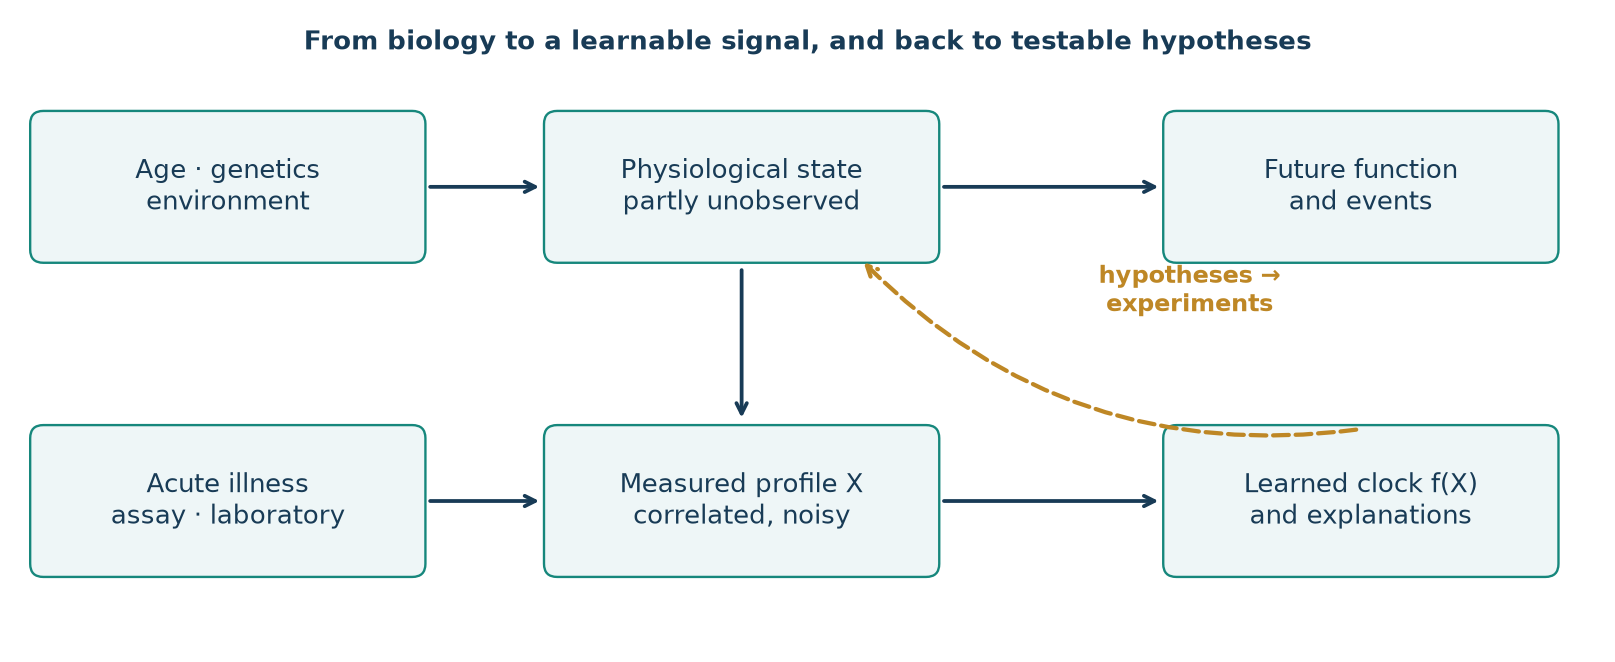
\includegraphics[width=0.88\linewidth]{01_conceptual_map.png}
\caption{Conceptual map (teaching schematic, not an identified causal model). Molecular profiles are noisy, correlated projections of a partially unobserved physiological state. Clocks and their explanations turn them into hypotheses that experiments can test.}
\label{fig:concept}
\end{figure}

\begin{table}[h]
\small
\begin{tabularx}{\linewidth}{@{}lXX@{}}
\toprule
\textbf{Challenge} & \textbf{Research opportunity it opens} & \textbf{Where treated}\\
\midrule
No ground-truth biological age & Outcome-anchored validation; disease cohorts as natural experiments & \cref{sec:gap}; \card{J6}\\
Redundant, correlated spectra & Biologically curated, well-conditioned representations & \cref{sec:conditioning}; \card{J4}\\
Regression to the mean & Reference-adjusted distortion; a theorem explaining the bias & \cref{sec:gap}\\
Laboratory and population shift & Transportable clocks with calibrated uncertainty & \cref{sec:conformal}; \card{J3}\\
Many outputs, one explanation? & The rigidity theorem for multi-output SHAP & \cref{sec:rigidity}; \card{J1}\\
\bottomrule
\end{tabularx}
\caption{Five challenges and five opportunities.}
\end{table}

\begin{translation}
\textbf{For mathematicians.} Aging is a partially observed dynamical system. A clock is a regression of calendar age on a high-dimensional, strongly collinear measurement vector. The interesting questions concern identifiability, stability, transport between populations and axiomatic explanation, not only accuracy.

\textbf{For geneticists.} A metabolic clock is a quantitative, repeatable phenotype that sits downstream of the genome and upstream of the clinic. It can be the target of genetic association studies, and its explanations can rank pathways for experimental follow-up.
\end{translation}

% =====================================================================
\section{State of the art: what the two papers achieved}
\label{sec:state}

\subsection{\PI\ The MetAge NMR clock and its disease maps}
\label{sec:P1}

\paragraph{Measurement and design} \REP
Each serum sample undergoes several NMR experiments (NOESY, CPMG, J-resolved and PGPE). J-resolved spectra support the quantification of 49 metabolites, and NOESY spectra are used to infer 25 routine clinical biomarkers, which \PI\ treats as semiquantitative proxies. Expert curation turns the initial 74 variables into a final set of 75. Haemoglobin, fructosamine and total cholesterol are discarded as redundant. GlycB is replaced by the ratio GlycB/GlycA, and total protein is decomposed into a non-albumin fraction. Further ratios are introduced, including urea/creatinine, BCAA/AAA, lactate/pyruvate and glutamine/glutamate \PI[pp.~4--5, 12--13].
The reference resource contains 29,390 individuals aged 7--106. Models are developed on an age- and sex-balanced subset of 8,640, balanced across five age strata of unequal width (7--30, 31--40, 41--50, 51--65, $>65$), with equal numbers in the first three and the two oldest adjusted to keep the overall sex balance, with 20\% held out and five-fold cross-validation on the rest. The learner is a TPOT-derived stack of Ridge and ExtraTrees after standardisation. An external Austrian cohort (121 participants, different country and laboratory) and 3,882 patients in eleven disease cohorts complete the design \PI[pp.~3--6, 12--13].

\begin{table}[h]
\centering\small
\begin{tabular}{@{}lrrr@{}}
\toprule
Representation & Test $r$ & Test RMSE (y) & Condition number $\kappa$\\
\midrule
NOESY bins & 0.93 & 6.5 & $\approx15{,}000$\\
CPMG & 0.92 & 6.8 & not reported\\
Raw FID (time domain) & 0.89 & 8.6 & not reported\\
Initial 74 biomarkers & 0.89 & 8.6 & $\approx38$\\
\rowcolor{teal!8}\textbf{Curated 75 biomarkers} & \textbf{0.88} & \textbf{8.7} & $\boldsymbol{\approx16}$\\
Automated IVDr reports (143 parameters) & 0.86 & 9.3 & $\approx180$\\
\bottomrule
\end{tabular}
\caption{\REP\ Accuracy--interpretability trade-off across representations \PI[pp.~4--5]. No uncertainty on the differences is reported.}
\label{tab:P1repr}
\end{table}

\begin{figure}[h]
\centering
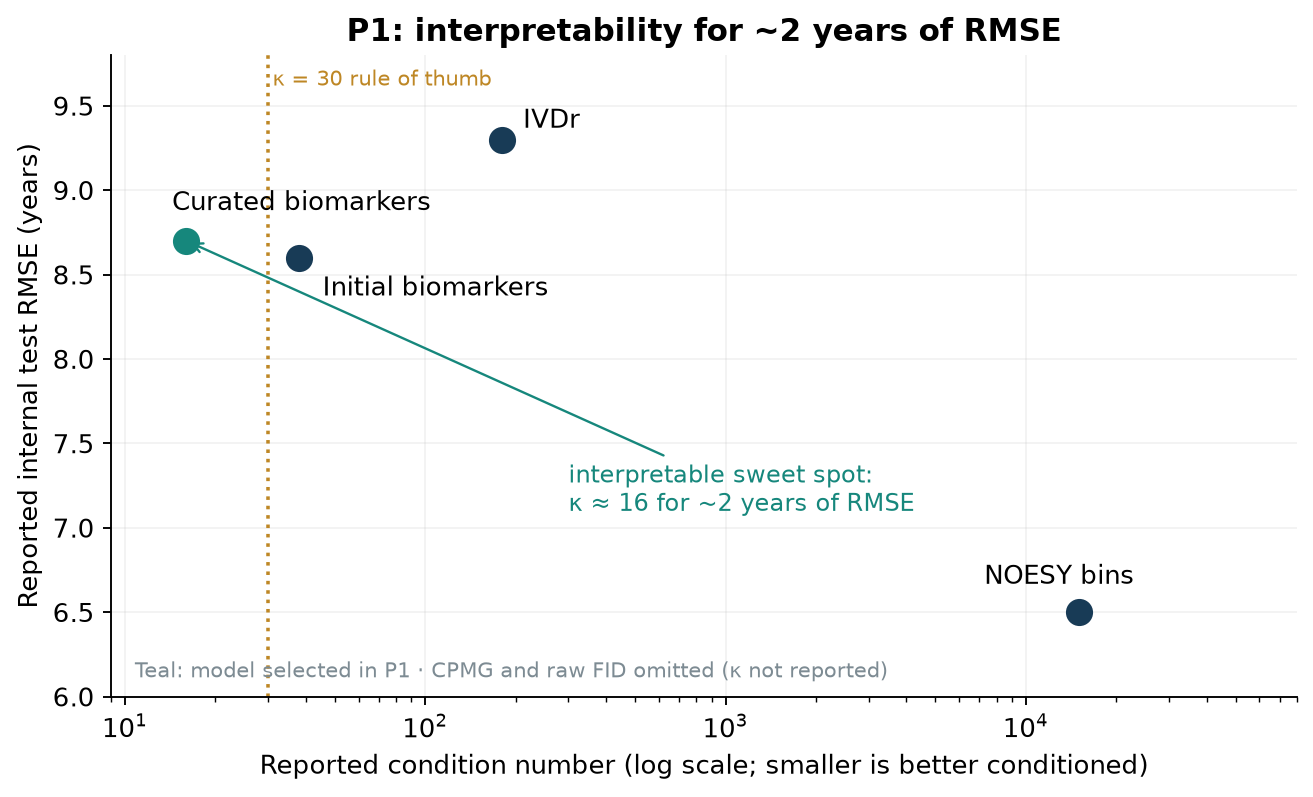
\includegraphics[width=0.72\linewidth]{02_p1_tradeoff.png}
\caption{The numbers of \cref{tab:P1repr} plotted as RMSE against condition number. The curated clock is well conditioned at a cost of about 2\,y of RMSE.}
\label{fig:tradeoff}
\end{figure}

\paragraph{Validation, sex and signature} \REP
On the internal test set $R=0.884$ and RMSE $8.68$\,y (\PI, Fig.~2a). The Austrian cohort gives $r=0.81$ and RMSE $12.2$\,y, against $0.89$ and $9.8$\,y for its age-matched reference. Its mean distortion is $1.9\pm9.7$\,y against $0\pm5.6$\,y, with Kolmogorov--Smirnov $p=0.10$ \PI[Fig.~2c, Fig.~4m, p.~6]. Statistically this is a failure to reject a difference, which is not the same as demonstrating equivalence (\cref{prob:transport}).
A single model works for both sexes: for females $r=0.909$ and RMSE $8.3$\,y, against $0.908$ and $8.2$\,y for a female-only model; for males $r=0.850$ and RMSE $9.0$\,y, against $0.877$ and $8.5$\,y for a male-only model \PI[p.~6].
Grouped SHAP ranks inflammation and immune activity first (16.9\%), followed by nitrogen homeostasis (13.4\%), energy metabolism (10.1\%) and structural integrity and systemic frailty (9.6\%) \PI[Fig.~3, p.~7]. The groups overlap: albumin, for instance, belongs to two of them. Albumin and ESR have the largest mean $|\mathrm{SHAP}|$ (3.1 and 2.4\,y), about twice that of alanine (1.6\,y) and 1,5-anhydrosorbitol (1.4\,y). \PI\ reads this as \emph{inflammaging} captured through time-integrated markers \PI[pp.~7, 10].

\begin{figure}[h]
\centering
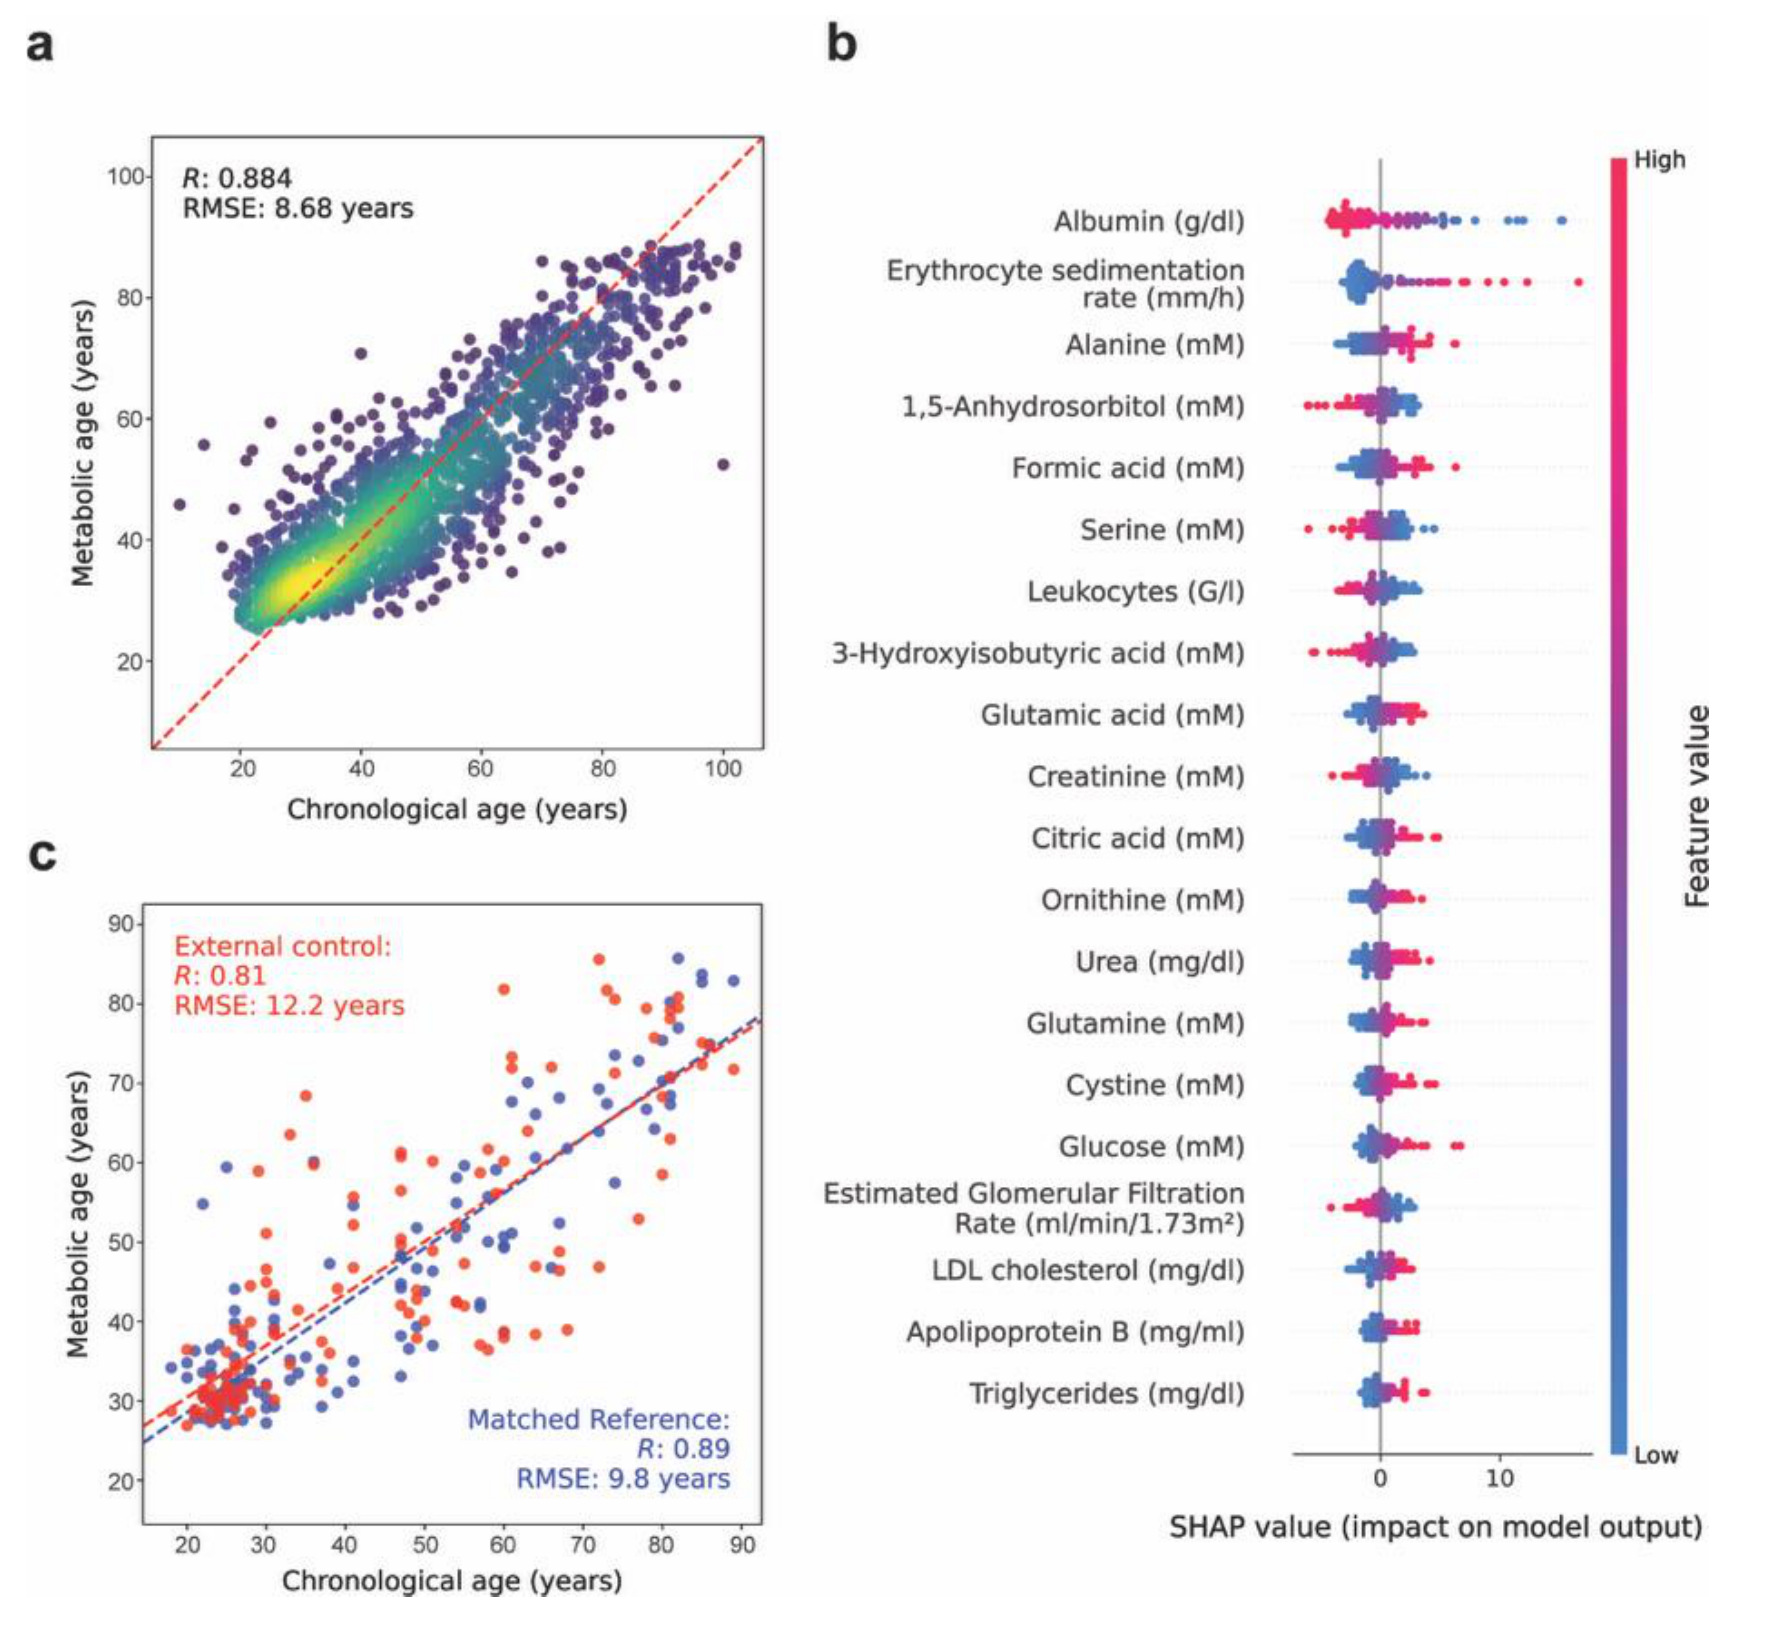
\includegraphics[width=\linewidth]{p1_original_figure2.png}
\caption{\REP\ Reproduced from \PI, Figure~2 (PDF p.~6). (a)~Internal test predictions. (b)~SHAP summary. (c)~External Austrian cohort (red) against its age-matched reference (blue). Credit: \PI\ authors.}
\label{fig:P1fig2}
\end{figure}

\paragraph{Disease maps} \REP
Metabolic distortion is the deviation from the reference regression line of predicted on chronological age. It is compared with age-matched references (also sex-matched for prostate cancer). All eleven comparisons are significant by the Kolmogorov--Smirnov test, and the two negative controls are not (\cref{fig:disease}). \PI\ also runs 1,000 negative-control resamplings of 1,000 healthy samples each, drawn from the 20,750 samples set aside during balancing \PI[pp.~6, 13].
A principal component analysis of the cohort $|\mathrm{SHAP}|$ profiles reveals three axes of distortion \PI[Fig.~5, pp.~9, 11]:
\begin{itemize}
\item a \emph{renal} axis (eGFR, and uremic toxins such as urea, myo-inositol and urate);
\item an \emph{inflammatory} axis (albumin, ESR, C-reactive protein), which isolates COVID-19 and influenza;
\item a \emph{strictly metabolic} axis (glutamic acid, sarcosine), characteristic of MASLD.
\end{itemize}
In long COVID the inflammatory signal has subsided, and glutamic acid and glucose dominate. \PI\ calls creatinine in CKD a \emph{false rejuvenator}. Elevated eGFR in the prospective CVD cohort (probably hyperfiltration) behaves the same way. These features lower the predicted age, yet no disease cohort shows a net younger metabolic age \PI[pp.~9--11].

\begin{figure}[h]
\centering
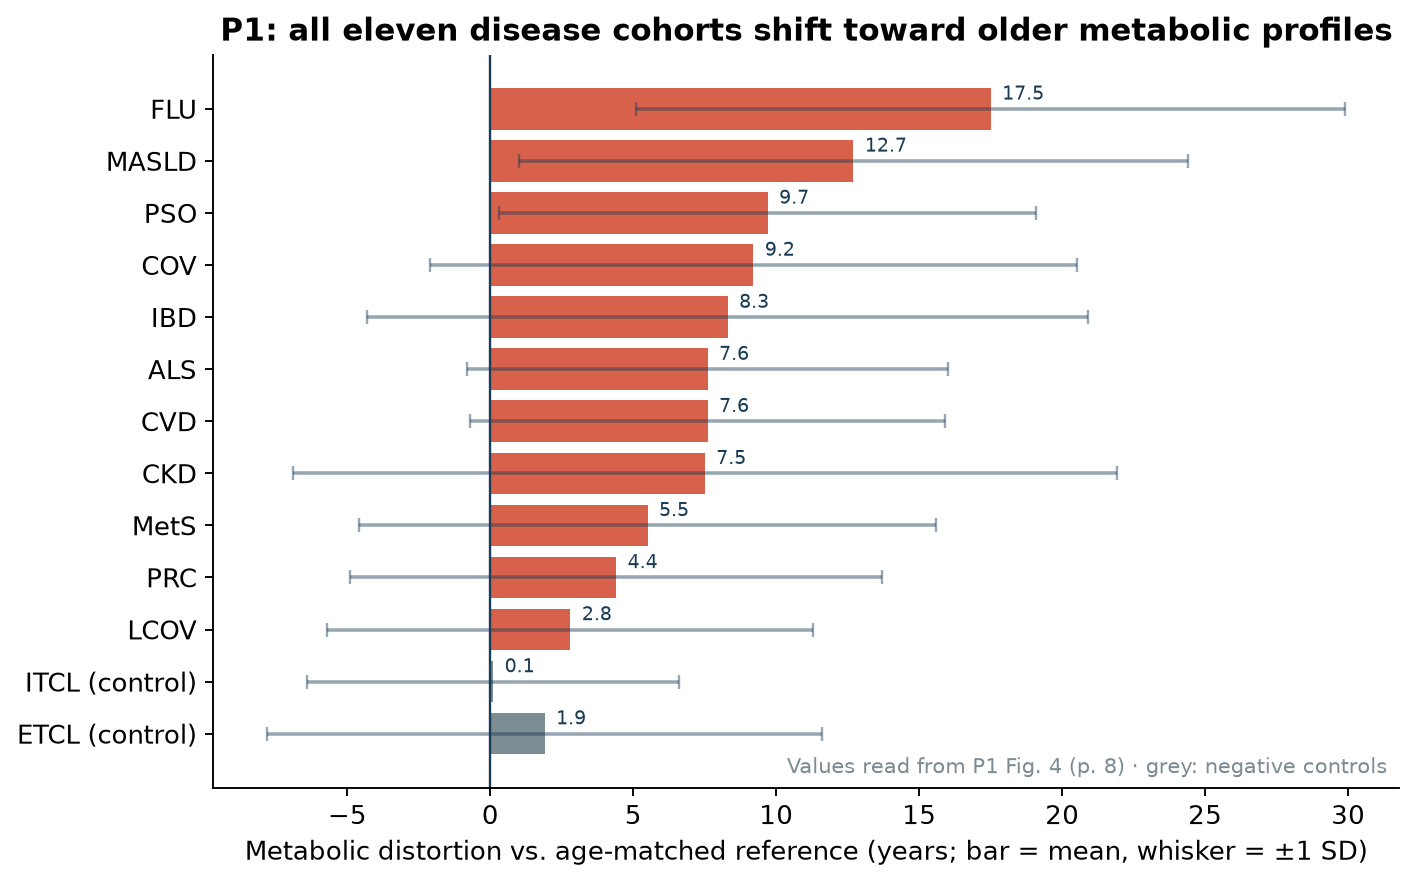
\includegraphics[width=0.84\linewidth]{11_p1_disease_distortion.png}
\caption{\REP\ Mean $\pm$ SD of metabolic distortion by cohort, as read from \PI, Fig.~4 (p.~8). The wide SDs show that a group shift is not individual predictive utility.}
\label{fig:disease}
\end{figure}

\begin{scope}
\PI\ names its own limitations and next steps \PI[p.~11]:
\begin{itemize}
\item the cohort is predominantly Caucasian;
\item false rejuvenators remain a conceptual challenge at the level of individual features;
\item future work should extend validation to more diverse populations, add longitudinal data and integrate further omics layers.
\end{itemize}
The disease findings are population-level associations. Individual prognostic value is the next test.
\end{scope}

\subsection{\PII\ Multi-output Shapley attribution}
\label{sec:P2}

\paragraph{Theory} \REP
\PII\ extends the Shapley axioms (efficiency, symmetry, dummy player, additivity) to vector-valued cooperative games $v:2^N\to\R^m$ (Def.~2.7). It proves that the unique admissible allocation is the coordinate-wise Shapley value (Thms~2.8--2.9, pp.~7--8), and that any rule coupling the outputs violates an axiom (Cor.~2.10). It then establishes Lipschitz stability of the operator in the game (Prop.~2.11) and in the predictor (Prop.~2.13). Appendix~B treats correlated Gaussian features in closed form and connects joint training with weak Pareto optimality \PII[pp.~22--25]. \Cref{sec:rigidity,sec:stability} restate these results precisely.

\paragraph{Experiment} \REP
The data are 15,931 complete observations with 75 numerical inputs, reduced by correlation-based pruning. There are three outputs: age, MetSCORE (a serum-NMR metabolic-syndrome risk index, Gil-Redondo et al.\ 2024) and recorded sex. The data are split 70/15/15 into training, validation and test sets. The models are a linear baseline M1 and a shared ReLU network M2 with regression and classification heads, trained with Adam (learning rate $10^{-3}$, batch 128, at most 200 epochs, early-stopping patience 20) on the unweighted sum of task losses. Explanations use DeepExplainer with 100 background samples \PII[§§3.1--3.3, pp.~11--14].

\begin{table}[h]
\centering\footnotesize\setlength{\tabcolsep}{3.5pt}
\begin{tabular}{@{}lccccc@{}}
\toprule
Model & Age $R^2$ & \shortstack{Age RMSE /\\MAE (y)} & \shortstack{MetSCORE\\$R^2$} & \shortstack{MetSCORE\\RMSE / MAE} & \shortstack{Sex accuracy /\\AUC / F1}\\
\midrule
M1 multi-output & 0.5614 & 8.9306 / 6.9946 & 0.7283 & 0.1343 / 0.0963 & 0.9373 / 0.9814 / 0.9462\\
M2 multi-output & 0.6206 & 8.3061 / 6.3454 & 0.8123 & 0.1116 / 0.0764 & 0.9485 / 0.9869 / 0.9559\\
M2 single-output & 0.6529 & 7.9438 / 6.0959 & 0.8173 & 0.1101 / 0.0745 & 0.9498 / 0.9849 / 0.9568\\
\bottomrule
\end{tabular}
\caption{\REP\ Predictive performance \PII[Tables~1--2, pp.~13--14]. Datasets, targets and splits differ from \PI, so the two papers' scores should not be ranked against each other.}
\label{tab:P2perf}
\end{table}

\paragraph{Computation and agreement} \REP
Three separate M2 models took 249.44\,s in total, and one joint M2 took 89.3678\,s, about $2.79\times$ faster. Peak RAM was 605.96 against 599.15\,MB. The hardware was a 14-core Intel Core Ultra 5 225H laptop with 32\,GB RAM running Python 3.13.5 \PII[Table~3, pp.~11, 14].
Between the joint and the separate M2 models, the feature-importance vectors have cosine similarities 0.9867, 0.9949 and 0.9740, and Spearman correlations 0.9460, 0.9003 and 0.8639, for age, MetSCORE and sex respectively \PII[Table~4, p.~16].
\PII\ reads the age signature through albumin and ESR (inflammation), 3-hydroxyisobutyrate, glucose and anhydrosorbitol, and urea and LDL. In Fig.~2, albumin ranks first for age and ESR seventh. For MetSCORE, glucose dominates, followed by HDL and LDL. For sex, erythrocyte counts, creatine/creatinine, urate, glycerol and SPC lead \PII[§3.4, Fig.~2, pp.~15--16].

\begin{figure}[h]
\centering
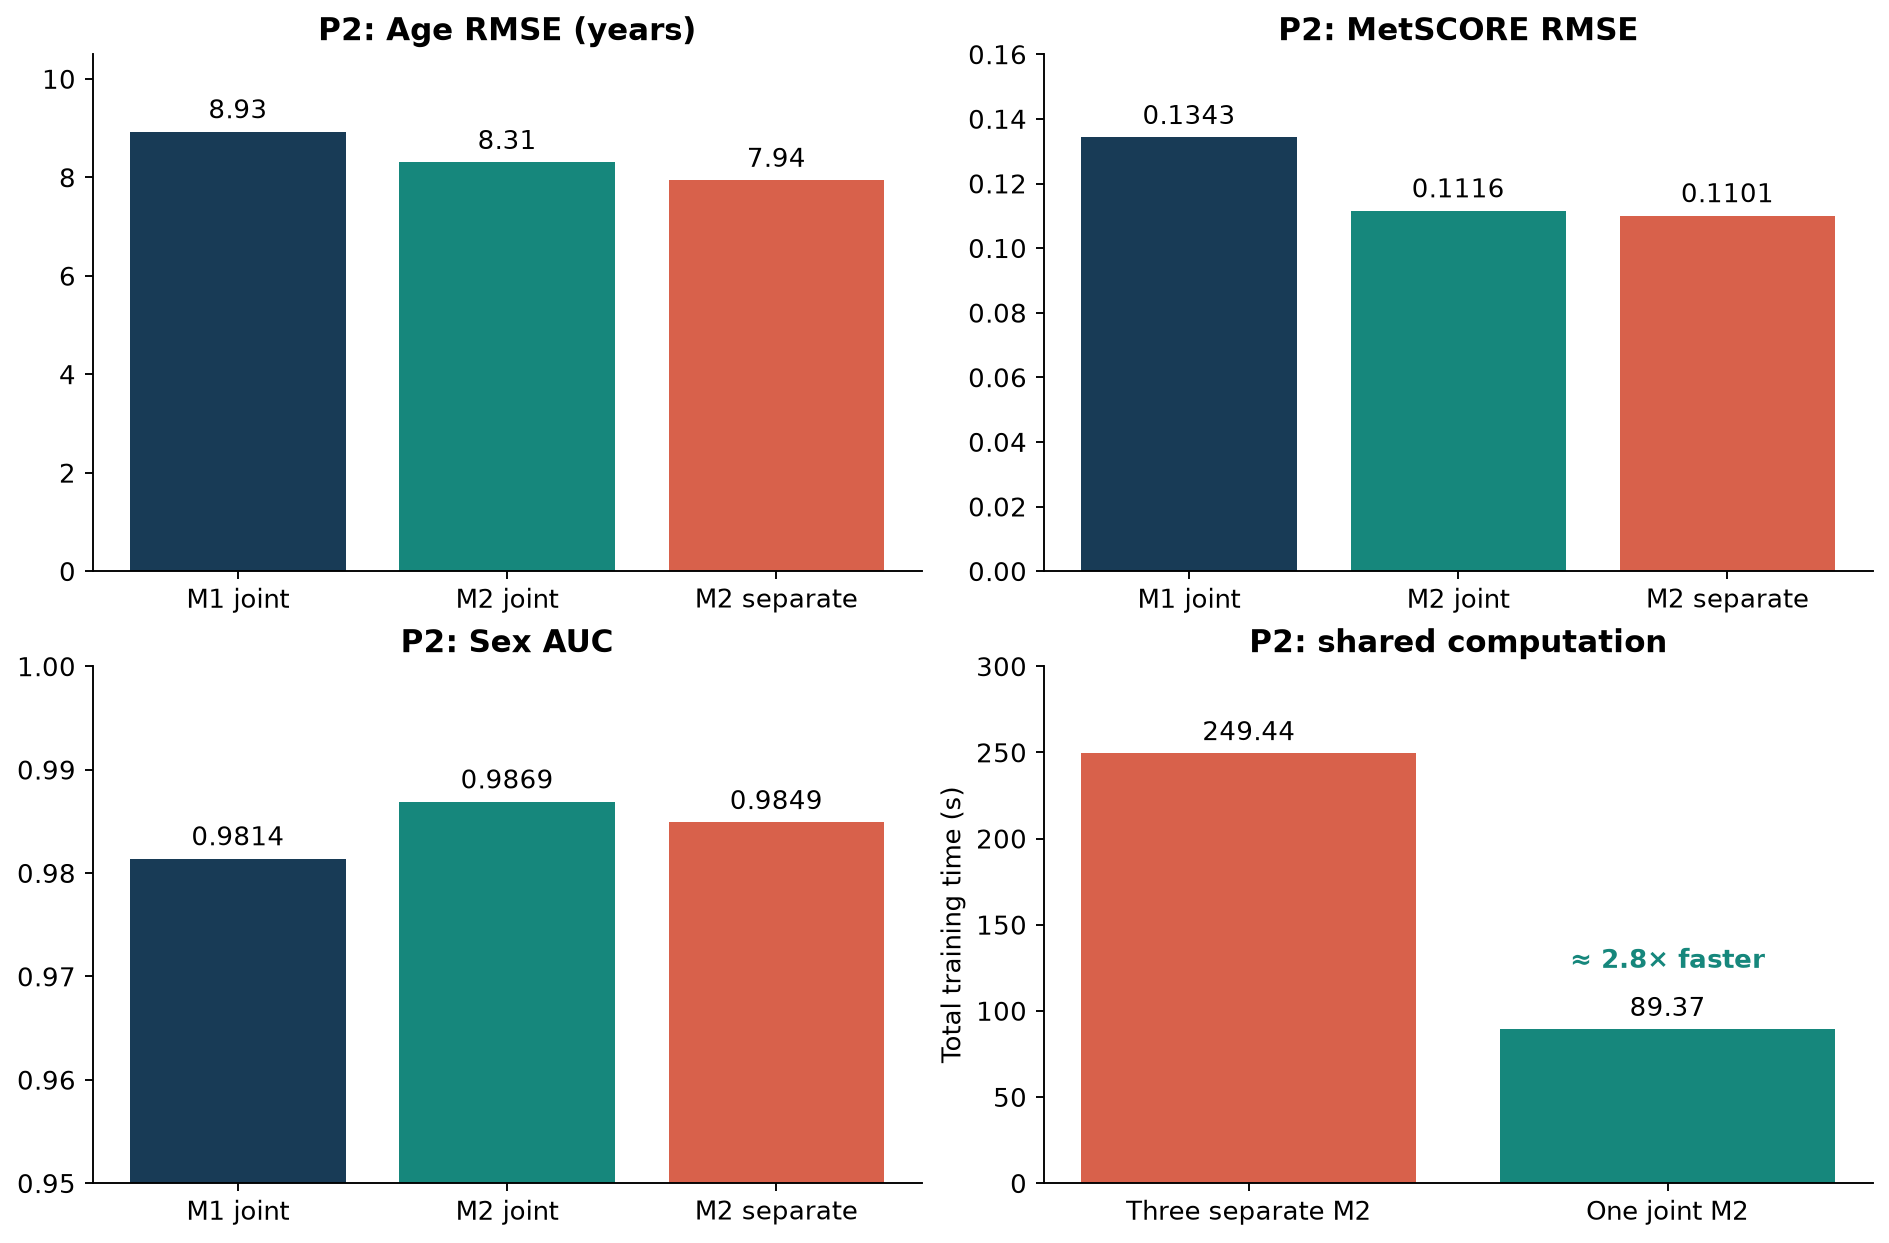
\includegraphics[width=0.78\linewidth]{10_p2_results.png}
\caption{\REP\ Key numbers of \PII, Tables~1--3. Note the truncated axis of the AUC panel: the sex-classification differences are in the third decimal.}
\label{fig:P2}
\end{figure}

\begin{scope}
\PII\ lists its own limitations \PII[p.~17]:
\begin{itemize}
\item it characterises existing attribution rather than proposing a new method;
\item rigidity holds for the classical axioms in full strength only;
\item the framework does not encode domain semantics.
\end{itemize}
The dedicated age model is more accurate than the joint one (RMSE 7.94 against 8.31\,y). \PII\ suggests that the shared model may weight metabolic over purely chronological signal. That is a hypothesis to be tested with independent outcomes.
\end{scope}

\subsection{Cross-paper synthesis}
\begin{itemize}
\item \textbf{Consistency.} Albumin leads both \PI's clock and \PII's age model, and ESR is among the top ten features of both \PII[Fig.~2, p.~15], on related serum-NMR data with different learners.
\item \textbf{Complementarity.} \PI\ supplies the phenotype, the curated representation and the disease maps. \PII\ supplies the axiomatic guarantee that multi-target models, such as several organ axes, age together with a risk score, or several disease states, can be explained rigorously output by output.
\item \textbf{A common open front.} Both papers stop where time, diversity and causality begin: longitudinal dynamics (\PI\ future work; \PII\ open problem~4), transport across populations, and the step from attribution to intervention.
\end{itemize}

\begin{conclusion}
\PI\ shows that interpretability can be engineered into a clock at a measurable and modest cost, and that the resulting explanations reveal disease-specific aging axes. \PII\ shows that explaining several outputs of one model is mathematically forced to be per output, so the explanations of a shared model remain per output. Together they make multi-output, interpretable metabolic clocks a well-posed next step.
\end{conclusion}

% =====================================================================
\section{A unified mathematical framework}
\label{sec:framework}

\begin{table}[h]
\centering\small
\begin{tabularx}{\linewidth}{@{}lX@{}}
\toprule
Symbol & Meaning\\
\midrule
$X\in\R^p$ & Measured features (metabolites, NMR-inferred biomarkers, ratios)\\
$A$ & Chronological age; $\pi$ its distribution in the training cohort\\
$C$ & Observed context: cohort, laboratory, recorded sex, medication\\
$Y$ & An independent outcome (event, function, mortality)\\
$B(t)$ & Latent, possibly multidimensional aging state (never observed)\\
$f(X)$ & A clock; $f^*(x)=\E[A\mid X=x]$ the least-squares optimum\\
$G=f(X)-A$ & Raw age gap\\
$m(a)=\E_{\mathrm{ref}}[f(X)\mid A=a]$ & Reference line; $D=f(X)-\widehat m(A)$ is the metabolic distortion\\
$v:2^N\to\R^m$ & A (vector) cooperative game on the features $N=\{1,\dots,p\}$\\
$\phi_j(v)$, $\Phi_j(v)$ & Scalar and vector Shapley allocation of feature $j$\\
$\mu$ & Background (reference) distribution defining ``missing'' features\\
\bottomrule
\end{tabularx}
\caption{Notation used throughout.}
\end{table}

\subsection{Clocks as learning problems}
A clock solves a regularised empirical-risk problem
\begin{equation}\label{eq:erm}
\widehat\theta\in\argmin_\theta\ \frac1n\sum_{i=1}^n\big(f_\theta(X_i)-A_i\big)^2+\lambda\,\Omega(\theta).
\end{equation}
Without penalty and over all square-integrable functions, the population optimum is
\begin{equation}\label{eq:fstar}
f^*(x)=\E[A\mid X=x]=\frac{\int a\,p(x\mid a)\,\pi(a)\,da}{\int p(x\mid a)\,\pi(a)\,da}.
\end{equation}
The target is therefore \emph{conditional chronological age in the reference population}. It depends on the age distribution $\pi$ of the training cohort. \PI's stratified balancing gives the five strata (of unequal width) roughly equal mass, so $\pi$ is the source age law reweighted by stratum. This is a modelling choice rather than neutral preprocessing. Over a restricted class the target becomes the $L^2$ projection of $f^*$ onto that class (when the class is closed and convex, for example a linear space; otherwise a best approximation), and $\lambda>0$ adds bias.

\subsection{Age gaps, regression to the mean and distortion}
\label{sec:gap}

If $\E[f(X)\mid A=a]=\alpha+\beta a$, then
$\E[G\mid A=a]=(\beta-1)(a-a_0)$ with crossing age $a_0=\alpha/(1-\beta)$. For $\beta<1$ people younger than $a_0$ look accelerated and people older than $a_0$ look decelerated, with no pathology at all (\cref{fig:gap}).

\begin{proposition}[Slope of the optimal clock] \NEW
\label{prop:gap}
Let $f^*=\E[A\mid X]$ and $R^2=\Var(f^*)/\Var(A)$. Then $\Cov(f^*,A)=\Var(f^*)$, and so:
\begin{enumerate}
\item the least-squares slope of $f^*$ on $A$ is $\beta=R^2$, which is less than $1$ unless $X$ determines $A$;
\item $\corr(f^*,A)^2=R^2$;
\item $\Cov(G,A)=-(1-R^2)\Var(A)$ and $\Cov(G,f^*)=0$.
\end{enumerate}
\end{proposition}
\begin{proof}
By the tower property, $\E[f^*A]=\E[f^*\,\E[A\mid X]]=\E[(f^*)^2]$ and $\E f^*=\E A$, so $\Cov(f^*,A)=\Var(f^*)$. Items (i)--(iii) follow by substitution. For example, $\Cov(G,A)=\Var(f^*)-\Var(A)$.
\end{proof}

\begin{proposition}[Calibration duality] \NEW
\label{prop:duality}
Let $s$ be any score with $r=\corr(s,A)>0$, and consider the affine recalibrations $g=a+bs$ with $\E g=\E A$.
\begin{enumerate}
\item The MSE-optimal recalibration has slope $r^2$ against age and RMSE $\sigma_A\sqrt{1-r^2}$.
\item The recalibration whose least-squares slope against age equals $1$ has RMSE $\sigma_A\sqrt{1-r^2}/r$.
\end{enumerate}
A clock therefore cannot be both least-squares optimal and free of age trend in its raw gap unless $r=1$. Among affine recalibrations, removing the trend costs exactly a factor $1/r$ in RMSE.
\end{proposition}
\begin{proof}
The slope of $g$ on $A$ is $b\,\Cov(s,A)/\Var A$. The MSE-optimal slope is $b^*=\Cov(s,A)/\Var s$, which gives slope $r^2$ against age. The unit-slope choice is $b_1=\Var A/\Cov(s,A)=b^*/r^2$. Since $\mathrm{MSE}(b)=\Var A-2b\Cov(s,A)+b^2\Var s$, substitution gives $\Var A\,(1-r^2)$ at $b^*$ and $\Var A\,(1-r^2)/r^2$ at $b_1$.
\end{proof}

\begin{remark}[Reading \PI's Figure~2a]
\PI\ reports no fitted slope. It reads the scatter against the identity line as showing minimal regression to the mean, relative to earlier NMR clocks. At $R=0.884$ a least-squares-calibrated clock has slope about $r^2\approx0.78$ against age. A slope near $1$ would instead indicate reverse calibration ($\E[f\mid A]\approx A$), which by \cref{prop:duality} costs about 13\% in RMSE among affine rescalings. Reporting the fitted slope would settle which convention a clock follows. The distortion $D$ is free of age trend under either choice, but not of scale. An affine recalibration $a+cf$ multiplies $D$ by $c$, so a unit-slope clock reports distortions $1/r^2\approx1.28$ times larger than a least-squares-calibrated one. Kolmogorov--Smirnov comparisons and cohort rankings are unaffected, but distortions stated in years depend on the convention. Making the choice explicit is a simple and valuable methodological contribution (\cref{prob:calibration}).
\end{remark}

\begin{figure}[h]
\centering
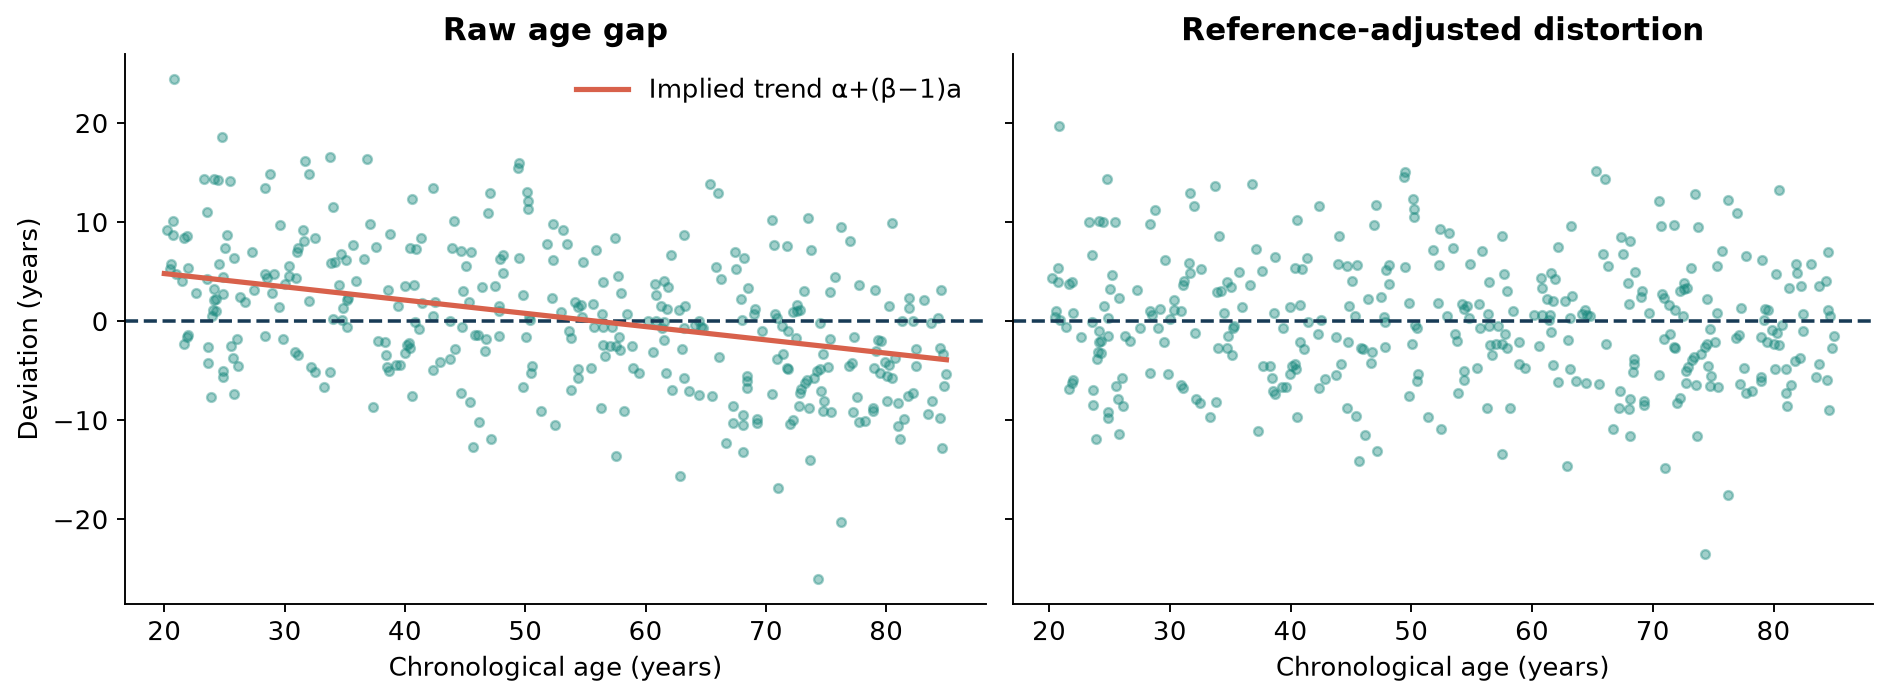
\includegraphics[width=0.86\linewidth]{05_gap_and_distortion.png}
\caption{Synthetic lab from the notebook. The raw gap inherits the trend $\alpha+(\beta-1)a$ of \cref{prop:gap}, while the reference-adjusted distortion does not.}
\label{fig:gap}
\end{figure}

\begin{translation}
Even a perfect learner makes young people look ``old'' and old people look ``young'' in the raw gap, because it predicts the \emph{average} age of people with your profile. That is why \PI's distortion, measured against a reference line, is the right quantity to map diseases. It is a mathematical requirement, not a cosmetic correction.
\end{translation}

\subsection{Conditioning and collinearity}
\label{sec:conditioning}
For a standardised design $Z=\sum_k\sigma_ku_kv_k^\top$ with $\kappa_2(Z)=\sigma_{\max}/\sigma_{\min}$,
\[
\Var(\widehat\beta_{\mathrm{OLS}})=\sigma^2\sum_k\frac{v_kv_k^\top}{\sigma_k^2},\qquad
\widehat\beta_{\mathrm{ridge}}=(Z^\top Z+\lambda I)^{-1}Z^\top y.
\]
For two near-duplicate markers the \emph{difference} direction $v_{\min}\propto(1,-1)$ is poorly determined, while the \emph{sum} is stable (\cref{fig:collinear}). Ridge replaces $1/\sigma_k$ by $\sigma_k/(\sigma_k^2+\lambda)$. \REP\ \PI\ observed exactly this mechanism in real data. Before curation, GlycA and GlycB both received high SHAP importance with opposite signs, which is physiologically implausible. Replacing GlycB by the ratio GlycB/GlycA and removing other redundancies lowered $\kappa$ to about 16 and gave ``stable and coherent'' SHAP distributions \PI[pp.~4--5]. The threshold $\kappa=30$ is a diagnostic convention (Belsley, Kuh and Welsch), not a theorem.

\begin{figure}[h]
\centering
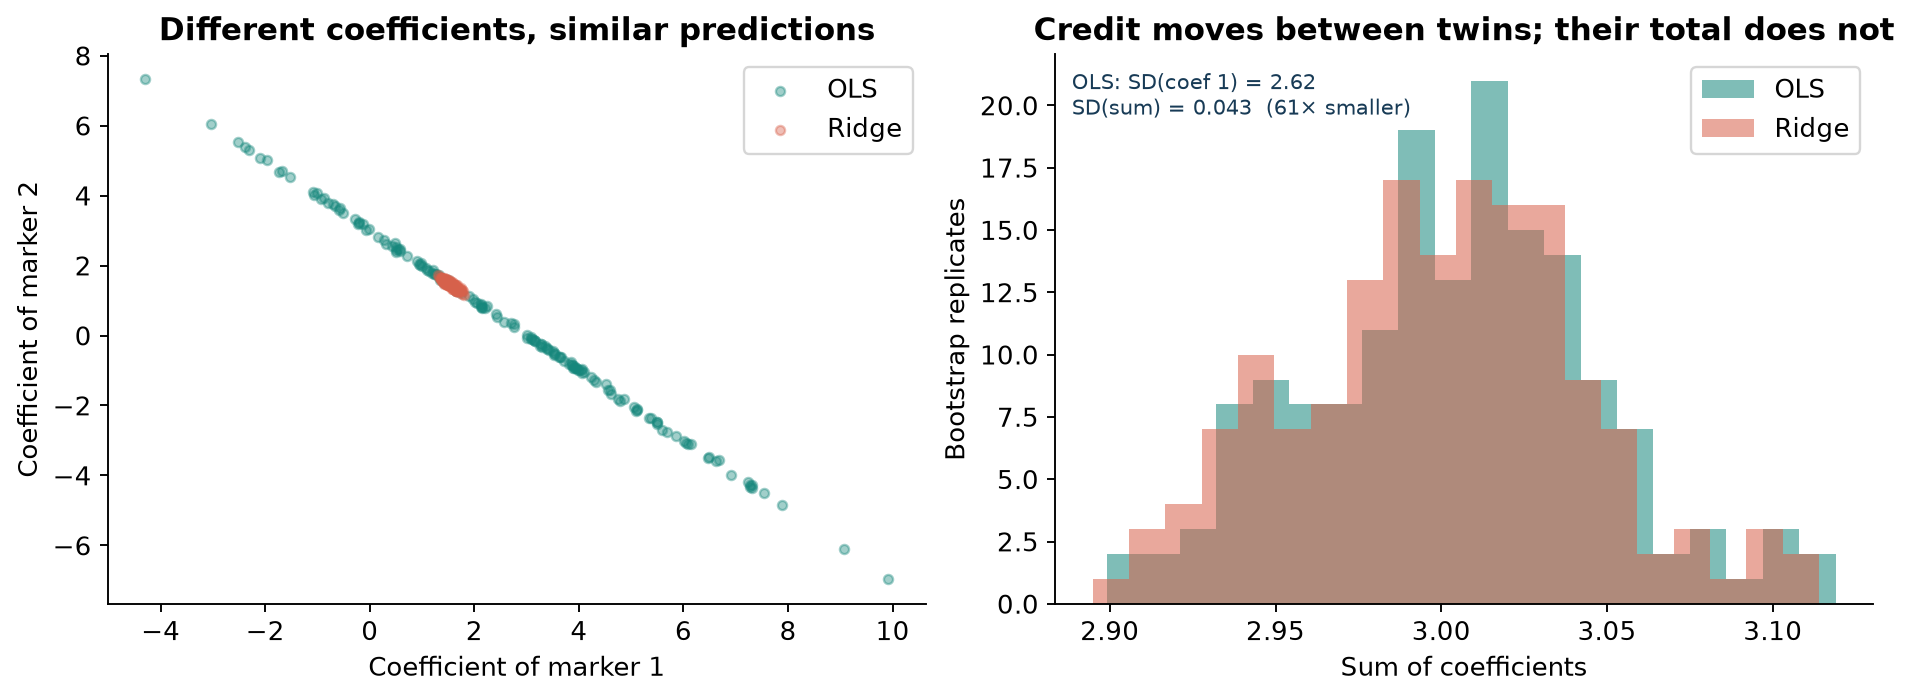
\includegraphics[width=0.86\linewidth]{07_collinearity.png}
\caption{Synthetic lab. Across bootstrap samples, OLS trades credit between two near-duplicate markers while their sum, and hence the prediction on the data manifold, stays stable. Ridge collapses the cloud.}
\label{fig:collinear}
\end{figure}

\subsection{Explanations as cooperative games}
For an individual $x$, \PII\ uses the conditional centred game \PII[eq.~(2.7), p.~10]
\[
v^{\mathrm{cond}}_x(S)=\E_\mu[f(X)\mid X_S=x_S]-\E_\mu[f(X)],
\]
and the Shapley value
\[
\phi_j(v)=\sum_{S\subseteq N\setminus\{j\}}\frac{|S|!\,(p-|S|-1)!}{p!}\big[v(S\cup\{j\})-v(S)\big],
\]
which is the unique rule satisfying efficiency, symmetry, dummy player and additivity \PII[Def.~2.3, Thms~2.4--2.5]. It reconstructs the prediction: $f(x)=\E_\mu f(X)+\sum_j\phi_j$ \PII[Prop.~2.12]. The \emph{marginal (interventional)} game instead averages $f(x_S,X_{-S})$ over the marginal law of the missing features. Marginal SHAP is ``true to the model'' and conditional SHAP is ``true to the data'' (Chen, Janizek, Lundberg and Lee 2020). Neither identifies the effect of an intervention.

\begin{example}[Proxy credit] \NEW
\label{ex:proxy}
Let $f(x)=x_1$ with $(X_1,X_2)$ standard bivariate Gaussian with correlation $\rho$. Then $v(\{1\})=x_1$, $v(\{2\})=\rho x_2$ and $v(N)=x_1$, so the conditional game gives $\phi=(x_1-\rho x_2/2,\ \rho x_2/2)$, while the marginal game gives $(x_1,0)$. The unused feature $x_2$ receives credit because it is not a dummy in the conditional game: revealing it changes the expected prediction. This is the phenomenon of \PII, Appendix~B.2: correlation couples feature contributions.
\end{example}

\paragraph{Grouped attributions.} With Harsanyi dividends $d_T=\sum_{S\subseteq T}(-1)^{|T|-|S|}v(S)$, one has $\phi_j=\sum_{T\ni j}d_T/|T|$. A pathway $H$ collects $\sum_Td_T\,|T\cap H|/|T|$, whereas the game in which whole groups are the players splits each dividend equally among the groups it touches. For a partition into groups, the two coincide whenever every interaction dividend lies within one group (in particular for additive games), and they differ in general. \PI's groups overlap, so its group scores are not of this form. \PI's pathway score is a sum of \emph{absolute} SHAP values \PI[p.~13]. It measures influence, not direction, and does not reconstruct the prediction.

\subsection{Vector games and the rigidity theorem}
\label{sec:rigidity}

\begin{theorem}[Rigidity; \PII, Thms~2.8--2.9, Cor.~2.10] \REP
Let $\Phi$ allocate vector games $v:2^N\to\R^m$ with $v(\varnothing)=0$, and suppose $\Phi$ satisfies efficiency, symmetry, dummy player and additivity, each imposed verbatim in $\R^m$. Then
\[
\Phi_j(v)=\big(\phi_j(v_1),\dots,\phi_j(v_m)\big)\qquad\text{for all }j\in N .
\]
Any allocation that couples outputs violates at least one of the four axioms.
\end{theorem}

\begin{proof}[Proof sketch (following \PII, App.~A)]
Every vector game is a finite sum $v=\sum_{T\ne\varnothing}\sum_kd_{T,k}\,u_Te_k$, where $u_T(S)=\mathbf 1[T\subseteq S]$ and $d_{T,k}$ are the coordinate-wise Harsanyi dividends. For the game $c\,u_Te_k$, players outside $T$ are dummies and receive $0$. Players in $T$ are symmetric and receive a common vector $a$. Efficiency gives $|T|a=c\,e_k$, so no other output coordinate appears. Additivity extends this to all games and yields the coordinate-wise Shapley formula. Conversely, the coordinate-wise rule satisfies the four axioms. \NEW\ \PII\ states additivity as linearity (Def.~2.3(iv)). Because the scaled basis games $c\,u_Te_k$ are handled directly, plain additivity already suffices. The dummy axiom is what excludes ``leaky'' rules, in which off-coordinate allocations cancel across players.
\end{proof}

\begin{corollary}[Linear readouts] \NEW
For every matrix $W\in\R^{q\times m}$, $\Phi(Wv)=W\,\Phi(v)$. A composite score built linearly from the outputs is explained by the same combination of per-output explanations, and one set of coalition evaluations serves every linear readout. A nonlinear readout, such as the sigmoid of a logit, requires a new game.
\end{corollary}

\begin{figure}[h]
\centering
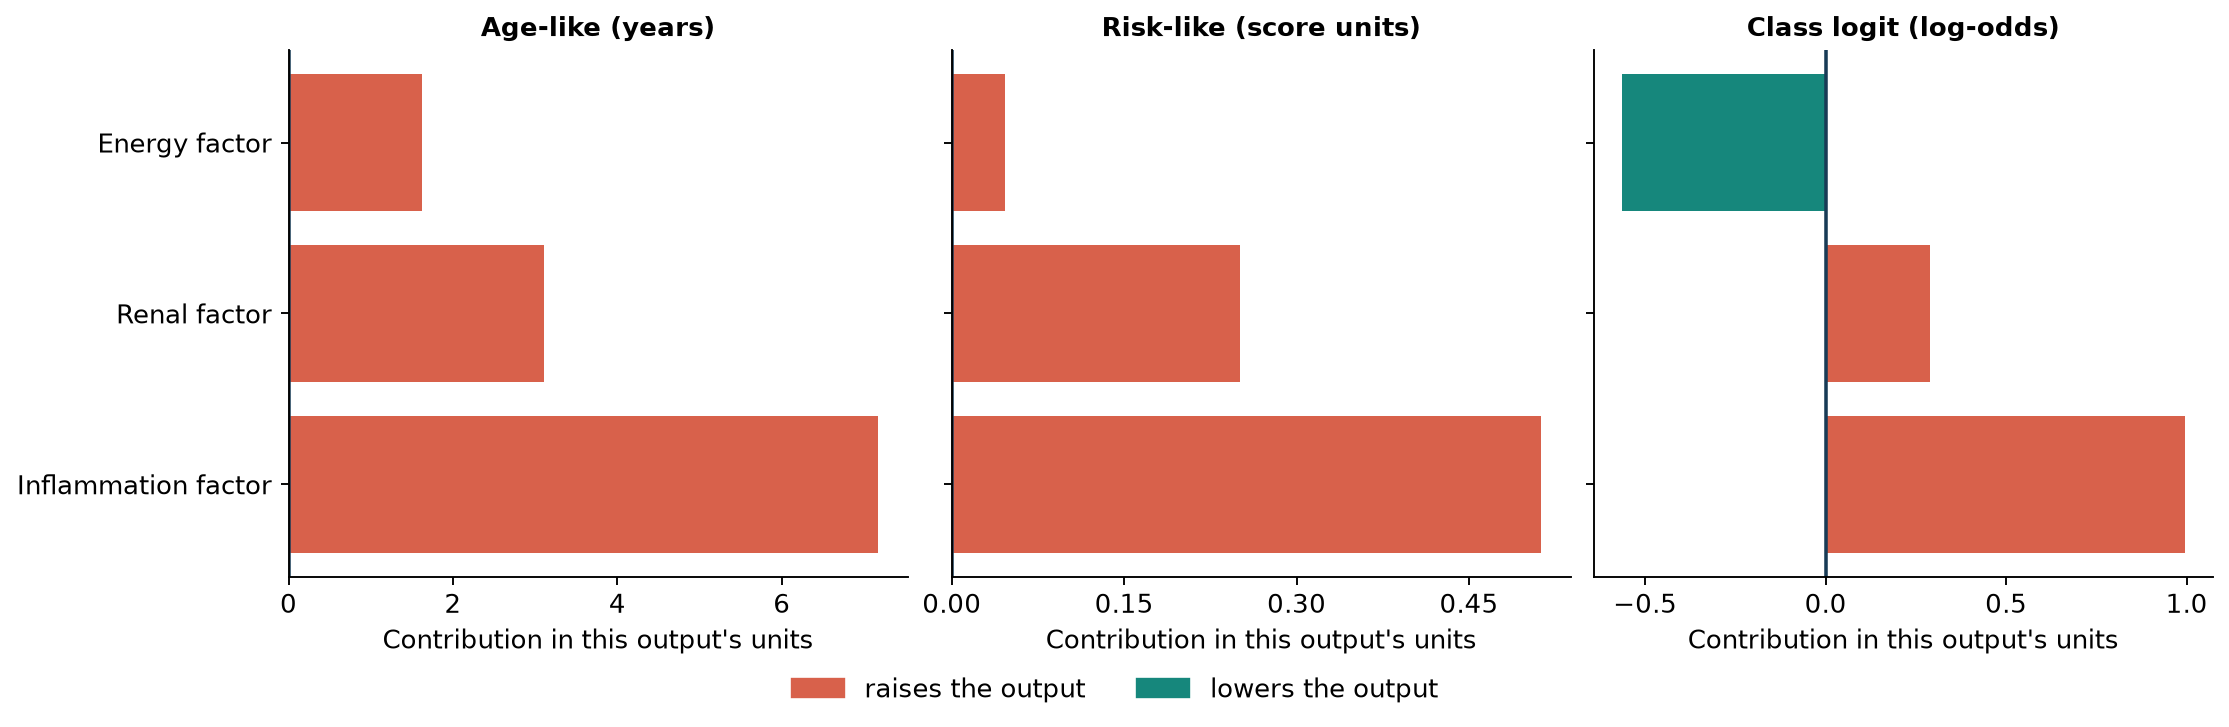
\includegraphics[width=0.92\linewidth]{09_vector_shap.png}
\caption{Synthetic lab. Three outputs (age-like, risk-like, class logit) of one linear model on three correlated Gaussian factors. Each output is explained in its own units, and none borrows credit from another.}
\end{figure}

\begin{scope}
Rigidity is conditional on the axioms. Coupling may become possible by scalarising efficiency, relaxing additivity or adding preference structure over outputs \PII[§2.4]. The theorem does not say that the outputs are independent, and it does not say that separately and jointly trained models have equal explanations. Those are different functions defining different games. The $2.79\times$ speed-up is an empirical finding, not a consequence of the theorem.
\end{scope}

\subsection{Stability}
\label{sec:stability}
\REP\ Let $\|\cdot\|_{A,\infty}$ be the largest feature/output entry of an allocation, $\|\cdot\|_{G,\infty}$ the largest coalition/output entry of a game, and $\|\cdot\|_{\Delta,\infty}$ the largest coalition increment. Then \PII[Prop.~2.11, p.~9]
\[
\|\Phi(u)-\Phi(v)\|_{A,\infty}\le\|u-v\|_{\Delta,\infty}\le2\,\|u-v\|_{G,\infty},
\]
and for predictors $f,g$ with a common background \PII[Prop.~2.13, p.~11]
\[
\|\Phi(f;x)-\Phi(g;x)\|_{A,\infty}\le\|v_f-v_g\|_{\Delta,\infty}\le2\,\|f-g\|_{L^\infty(\mu)} .
\]
\NEW\ In the game bound of Prop.~2.11 the constant sharpens to $2-1/p$, that is $\|\Phi(u)-\Phi(v)\|_{A,\infty}\le(2-1/p)\|u-v\|_{G,\infty}$, because the empty-coalition increment has weight $1/p$ and involves a single game value ($v(\varnothing)=0$). This does not improve the predictor bound $2\|f-g\|_{L^\infty(\mu)}$. For the conditional game, closeness of $f$ and $g$ on the data distribution suffices. The $L^\infty(\mu)$ bound holds for $\mu$-almost every $x$, and at every $x$ in the support when the conditional laws admit a continuous version. For the marginal game one needs $\sup|f-g|$ over the product of marginals, which lies partly \emph{off} the data manifold. Two clocks that agree on real profiles can therefore explain very differently.

\subsection{Uncertainty: split conformal prediction}
\label{sec:conformal}
With a frozen predictor $f$, calibration scores $s_i=|A_i-f(X_i)|$ and $q$ the $\lceil(n_{\mathrm{cal}}+1)(1-\alpha)\rceil$-th smallest score, exchangeability gives
$1-\alpha\le P(|A_{\mathrm{new}}-f(X_{\mathrm{new}})|\le q)\le1-\alpha+1/(n_{\mathrm{cal}}+1)$, the upper bound holding without ties (Angelopoulos and Bates 2021). This is marginal coverage for \emph{chronological} age. Exact conditional coverage at every $x$ is impossible distribution-free (Vovk 2012; Barber et al.\ 2021), and the interval says nothing about a person's ``true'' biological age.

\subsection{Joint training}
\PII\ minimises $\mathrm{MSE}(\widehat A,A)+\mathrm{MSE}(\widehat M,M)+\ell_{\mathrm{BCE}}(\widehat\ell,S)$ with equal weights and standardised inputs \PII[pp.~12--13]. At the reported errors, an unscaled age MSE ($\approx8.31^2\approx69$\,y$^2$) exceeds the MetSCORE MSE ($\approx0.112^2\approx0.012$) by a factor of about 5,500. Target scaling therefore decides what ``equal weights'' means. This connects to adaptive weighting schemes (uncertainty weighting, GradNorm, MGDA-type Pareto methods) and to the weak-Pareto view of \PII, App.~B.3.

% =====================================================================
\section{Evidence ledger: established, supported, open}
\label{sec:ledger}

\begin{longtable}{@{}p{0.43\linewidth}p{0.13\linewidth}p{0.36\linewidth}@{}}
\toprule
\textbf{Claim} & \textbf{Status} & \textbf{What would upgrade it}\\
\midrule\endhead
Serum NMR encodes chronological age ($r\approx0.88$--$0.93$) \PI & Established & ---\\
Curation lowers $\kappa$ to $\approx16$ and stabilises SHAP \PI & Established (one resource) & Whole-pipeline bootstrap; second laboratory\\
Clock transfers to another laboratory \PI & Supported; accuracy degrades & Larger external cohorts; equivalence tests (\cref{prob:transport})\\
All 11 disease cohorts shift older \PI & Established at group level & Individual-level discrimination; prospective designs\\
Three distortion axes \PI & Supported & Stability of the PCA axes under resampling (\cref{prob:geometry})\\
Pre-event acceleration in CVD ($n=59$) \PI & Promising & Larger prospective cohort; value beyond standard risk scores (\card{J6})\\
Remission reduces distortion (IBD) \PI & Association & Within-person longitudinal data (\card{J2})\\
Coordinate-wise attribution is forced by the axioms \PII & Theorem & ---\\
Joint training saves computation \PII & Established (one setting) & Multi-seed, multi-hardware benchmark (\card{J1})\\
Joint and separate explanations agree \PII & Empirical & Data-driven certificate (\card{J4})\\
Shared models capture ``more biology'' \PII & Hypothesis & Independent outcomes\\
Metabolic distortion has a genetic component & Open & Genotyped cohorts (\card{J5})\\
\bottomrule
\end{longtable}

% =====================================================================
\section{Open problems for mathematicians}
\label{sec:math}

The first five problems are the open problems stated in \PII, §4 (pp.~16--18), in our wording. The remaining ones are \PROP\ proposals motivated by \PI\ and by the experiments of \PII.

\begin{problem}[Beyond the Shapley axioms; \PII\ OP1]\label{prob:beyond}
Characterise allocation rules for vector games that satisfy symmetry, dummy player and additivity together with a \emph{weakened} efficiency, for example $\langle w,\sum_j\Phi_j(v)\rangle=\langle w,v(N)\rangle$ for $w$ in a cone of preferences. Which extra axiom (covariance under output reparametrisation, or an interaction index across outputs) singles out a unique coupled rule? A natural first result is a complete description of the solution set as an affine space over the coordinate-wise rule.
\end{problem}

\begin{problem}[Correlation-aware estimation; \PII\ OP2]\label{prob:estimation}
Permutation-sampling estimators share coalition evaluations across outputs. Quantify the variance reduction obtainable from control variates built from correlated outputs, as a function of the output correlation matrix. Derive optimal sample allocation, and benchmark against exact small games using the notebook's \texttt{exact\_shapley}.
\end{problem}

\begin{problem}[Pareto structure; \PII\ OP3]\label{prob:pareto}
For scalarised training $\theta^*(w)\in\argmin_\theta\sum_kw_k\mathcal L_k(\theta)$, study the map $w\mapsto\Phi(f_{\theta^*(w)};x)$ along the weak Pareto front. Combine \PII\ Prop.~2.13 with the sensitivity of $\theta^*(w)$ to obtain Lipschitz bounds on how explanations move along the front. Can Pareto-stationarity conditions be read in attribution space?
\end{problem}

\begin{problem}[Dynamic SHAP; \PII\ OP4]\label{prob:dynamic}
For time-dependent predictors (recurrent networks, controlled ODEs $\dot x=F(x,u)$), define games whose players are (feature, time) pairs or trajectory segments, satisfying efficiency along trajectories and additivity. Relate them to adjoint sensitivities (Pontryagin) and to path-integral attributions (Aumann--Shapley, integrated gradients). This is the bridge between explainability and control theory announced in \PII, and the mathematical core of \card{J2}.
\end{problem}

\begin{problem}[High-dimensional computation; \PII\ OP5]\label{prob:highdim}
Extend spectral or general-Fourier representations of SHAP (Morales, arXiv:2511.00185) to vector outputs. The approximations should preserve efficiency exactly and come with rigorous error bounds. Use the Gaussian closed forms of \PII, App.~B as test cases.
\end{problem}

\begin{problem}[Certified explanation agreement]\label{prob:certificate}
\PROP\ Turn the Table~4 agreement of \PII\ into a certificate. Estimate $\|v_f-v_g\|_{\Delta,\infty}$ from data with concentration bounds, and add a bound on the approximation error of the explainer (DeepExplainer approximates a background-based game, and \PII\ notes that its results ``apply to the exact Shapley operator''). A second target is a stability theory for \emph{rankings} (Spearman), not only for values.
\end{problem}

\begin{problem}[Which calibration should a clock satisfy?]\label{prob:calibration}
\PROP\ \Cref{prop:duality} shows a sharp trade-off between forward calibration ($\E[A\mid f]=f$) and reverse calibration ($\E[f\mid A]=A$). Extend it beyond affine rescalings and to nonlinear reference lines. Study how the training age law $\pi$ in \eqref{eq:fstar} moves the target, and derive the bias of distortion when a clock trained under one $\pi$ is read in a population with another.
\end{problem}

\begin{problem}[Transport and equivalence]\label{prob:transport}
\PROP\ Develop shift-aware uncertainty for clocks, such as weighted conformal prediction under covariate shift or optimal-transport alignment of assays across laboratories. Pair it with \emph{equivalence tests} (for instance TOST on distortion distributions) that can positively demonstrate transport, replacing ``failure to reject'' at $n=121$.
\end{problem}

\begin{problem}[Geometry of disease signatures]\label{prob:geometry}
\PROP\ Is disease distortion a low-dimensional object? Study the geometry of cohort and individual $|\mathrm{SHAP}|$-profile embeddings, the stability of \PI's three PCA axes under bootstrap and background changes, and signed versus absolute aggregations. Develop context-conditional games that flag \emph{false rejuvenators}, that is, features whose contribution reverses sign between the reference and a disease context.
\end{problem}

\begin{problem}[Identifiability of a latent aging state]\label{prob:latent}
\PROP\ Consider the state-space model
\[
B_i(t+\Delta)=F_\theta\big(B_i(t),U_i(t),\Delta\big)+\eta_i(t),\qquad X_i(t)=H_\psi\big(B_i(t),C_i(t)\big)+\epsilon_i(t).
\]
Under which structural constraints and sampling designs are $B$, $F_\theta$ or intervention effects identifiable from repeated measurements, age and outcomes? A multidimensional (organ-wise) $B$ is the natural setting for \card{J1}.
\end{problem}

% =====================================================================
\section{Open problems for genetics, metabolomics and clinical biology}
\label{sec:bio}

\begin{problem}[Diverse reference populations]\label{prob:diverse}
\REP\ \PI\ calls for validation across more diverse populations, since its cohort is predominantly Caucasian \PI[p.~11]. Recruit and harmonise multi-ancestry reference data, and quantify how the reference line $m(a)$ and the signature change.
\end{problem}

\begin{problem}[Trait or state?]\label{prob:trait}
\REP/\PROP\ \PI\ calls for longitudinal data. How much of an individual's distortion persists after recovery from acute illness? Obtain repeated samples through illness and recovery (building on the IBD remission signal) and estimate the within-person, technical and between-person variance components.
\end{problem}

\begin{problem}[Genetic architecture of metabolic distortion]\label{prob:genetic}
\PROP\ Is distortion heritable? Run a genome-wide association study of distortion and of its axis-specific components, and use Mendelian randomisation under stated assumptions (pleiotropy, population structure, selection). A high SHAP rank alone never establishes a genetic mechanism.
\end{problem}

\begin{problem}[Multi-omics integration]\label{prob:omics}
\REP/\PROP\ \PI\ calls for additional omics layers. Do methylation, proteomic and metabolic clocks measured on the same samples capture the same or complementary aging? Which layer best anticipates outcomes?
\end{problem}

\begin{problem}[Organ-specific metabolic ages]\label{prob:organ}
\PROP\ Can the renal, inflammatory and hepatic-metabolic axes of \PI\ be turned into separate, validated organ-level metabolic ages? This follows the multi-organ aging literature cited in \PII\ (§1.2; Tian et al.\ 2023).
\end{problem}

\begin{problem}[Mechanisms behind the signature]\label{prob:mechanism}
\PROP\ Design experimental follow-up of the leading signals: the albumin--ESR axis as a time-integrated inflammaging readout, glutamic acid as a hub in MASLD, the shift toward glutamate and glucose in long COVID, and the context-dependent meaning of creatinine and eGFR.
\end{problem}

\begin{perspective}
The biological problems supply the data that make the mathematical problems concrete. Longitudinal samples feed \cref{prob:dynamic,prob:latent}, multi-laboratory data feed \cref{prob:transport}, and organ-wise targets feed \cref{prob:beyond,prob:pareto}. The mathematical problems in turn supply the guarantees that make the biological conclusions defensible.
\end{perspective}

% =====================================================================
\section{Joint flagship projects}
\label{sec:joint}

Each card is a \PROP. The partner roles are indicative and are to be agreed by the group.

\begin{projectcard}{J1}{A multi-axis metabolic clock with rigorous per-output explanations}
\phantomsection\label{card:J1}
\field{Question} Can one shared model predict chronological age together with renal, inflammatory and hepatic-metabolic axis scores (and MetSCORE), while each output keeps a stable, interpretable explanation?
\field{Hypothesis} Shared representations improve the weaker targets at negligible cost to age accuracy. By the rigidity theorem, explanations stay per output.
\field{Data} The \PI\ reference resource and disease cohorts, with axis targets defined \emph{a priori} from clinical variables rather than from the same SHAP analysis.
\field{Methods} Multi-task networks with loss scaling and Pareto methods (\cref{prob:pareto}), exact small-game validation of the explainer, and a multi-seed benchmark.
\field{Deliverables} An open benchmark and a methods paper, with a biomedical companion paper on organ-level metabolic aging.
\field{Roles} Biology: axis definitions, cohort curation, interpretation. Mathematics: architecture, loss balancing, attribution guarantees.
\field{Risks} Circularity if axis targets are built from the input biomarkers (the same issue arises for MetSCORE, which \PII\ describes as a weighted combination of blood-based biomarkers, p.~11).
\field{Notebook entry point} §9 (rigidity lab, \texttt{multi\_output\_figure}) and the joint-learning lab.
\end{projectcard}

\begin{projectcard}{J2}{Trait or state: dynamics of metabolic distortion and dynamic SHAP}
\phantomsection\label{card:J2}
\field{Question} How does distortion evolve within a person through illness, recovery and treatment, and how should a time-dependent prediction be explained?
\field{Hypothesis} Distortion decomposes into a persistent trait and transient, axis-specific states. The IBD remission signal is the first evidence \PI[p.~8].
\field{Data} Repeated serum samples with clinical metadata. The collaboration still needs to establish which existing cohorts have them.
\field{Methods} Mixed-effects and state-space models (\cref{prob:latent}), and dynamic Shapley games with trajectory efficiency (\cref{prob:dynamic}).
\field{Deliverables} A variance-decomposition paper (biology), a dynamic-SHAP theory paper (mathematics), and a joint paper applying it to recovery trajectories.
\field{Risks} Few within-person samples; confounding by treatment.
\end{projectcard}

\begin{projectcard}{J3}{Transportable clocks across laboratories and populations}
\phantomsection\label{card:J3}
\field{Question} Can a metabolic clock be shown to transfer, rather than merely not fail, across laboratories, ancestries and assay versions?
\field{Data} Additional external cohorts. Multi-ancestry recruitment (\cref{prob:diverse}). Replicate samples measured in several laboratories.
\field{Methods} Covariate-shift conformal prediction, optimal-transport assay alignment, equivalence testing, and subgroup calibration (\cref{prob:transport}).
\field{Deliverables} A preregistered external validation with cohort-level intervals, and a methods paper on certified transport.
\end{projectcard}

\begin{projectcard}{J4}{Certified and reproducible explanations}
\phantomsection\label{card:J4}
\field{Question} Which pathway-level statements survive resampling, background changes, explainer approximation and a new laboratory?
\field{Methods} Whole-pipeline bootstrap, conditional-versus-marginal sensitivity, grouped games through Harsanyi dividends, and data-driven bounds on $\|v_f-v_g\|_{\Delta,\infty}$ (\cref{prob:certificate}).
\field{Deliverables} A ``pathway stability report'' standard, applied to \PI's signature and to \PII's Table~4, and a theory paper on certified attribution.
\end{projectcard}

\begin{projectcard}{J5}{From metabolic age to the genome}
\phantomsection\label{card:J5}
\field{Question} Does metabolic distortion, overall or axis-specific, have a heritable component, and which loci and pathways drive it?
\field{Data} Genotyped participants with serum NMR. Whether such subsets exist within the consortium is to be established.
\field{Methods} GWAS of distortion and its axes, genetic correlation with disease, Mendelian randomisation with sensitivity analyses, and correction for family and population structure.
\field{Deliverables} A genetics paper; if positive, a mechanistic follow-up (\cref{prob:mechanism}).
\field{Risks} Power; the clock's inputs may be under direct genetic control, which confounds the interpretation of distortion.
\end{projectcard}

\begin{projectcard}{J6}{Outcome-anchored validation}
\phantomsection\label{card:J6}
\field{Question} Does distortion add predictive value beyond age and standard clinical risk scores for future events, function or mortality?
\field{Data} Prospective cohorts with follow-up. \PI's CVD cohort ($n=59$) is the pilot signal.
\field{Methods} Prespecified survival models with censoring, discrimination and calibration increments, and decision-curve analysis.
\field{Deliverables} A clinical-validation paper, which is the decisive test of ``biological'' age.
\end{projectcard}

\begin{projectcard}{J7}{Context-aware attribution and false rejuvenators}
\phantomsection\label{card:J7}
\field{Question} Can attribution detect when a feature's meaning reverses between the reference and a disease context (creatinine in CKD, which \PI\ calls a false rejuvenator; elevated eGFR in probable hyperfiltration)?
\field{Methods} Disease-conditional backgrounds and games, out-of-support detection, and signed SHAP differences against matched controls (\cref{prob:geometry}).
\field{Deliverables} A methods paper that turns \PI's stated conceptual challenge into a diagnostic tool.
\end{projectcard}

% =====================================================================
\section{Candidate papers}
\label{sec:papers}

\begin{longtable}{@{}p{0.05\linewidth}p{0.36\linewidth}p{0.12\linewidth}p{0.17\linewidth}p{0.22\linewidth}@{}}
\toprule
\# & Working title (\PROP) & Type & Depends on & Venue type\\
\midrule\endhead
1 & Forward and reverse calibration of aging clocks: a sharp trade-off & Short methods & \cref{prop:duality}; existing data & Biostatistics / aging methods\\
2 & Vector Shapley values beyond classical efficiency & Theory & \cref{prob:beyond} & Mathematics of data science\\
3 & Variance-reduced estimation of multi-output SHAP & Theory + numerics & \cref{prob:estimation,prob:highdim} & ML / computational maths\\
4 & Dynamic Shapley values and control & Theory & \cref{prob:dynamic} & Control / applied maths\\
5 & Certified agreement of explanations across models & Theory + application & \cref{prob:certificate} & Mathematics of data science\\
6 & A multi-axis interpretable NMR metabolic clock & Application & J1 & Aging / metabolomics\\
7 & Trait and state components of metabolic aging & Application & J2 data & Aging / clinical\\
8 & External validation of an NMR clock across laboratories & Application & J3 data & Clinical chemistry / epidemiology\\
9 & Genetic architecture of metabolic distortion & Application & J5 data & Genetics\\
10 & Detecting false rejuvenators with context-aware attribution & Methods & J7 & Bioinformatics\\
\bottomrule
\end{longtable}

Papers~1, 2, 3 and 10 can start immediately with existing data or pure theory. Papers~7--9 depend on data availability that the group needs to confirm first (\cref{sec:plan}).

% =====================================================================
\clearpage
\section{Standards for evaluation and reporting}
\label{sec:standards}

\paragraph{Evaluation design.}
\begin{itemize}
\item Split first by the unit of independence (person, family or cohort).
\item Fit imputation, scaling, feature selection and any upstream predictor inside training folds. In a spectrum $\to$ inferred biomarker $\to$ age stack, check overlap at both stages.
\item Fit the reference line on separate reference data, and open the test set once.
\item Check age-dependent formulas (for example some eGFR definitions) for encoded age information.
\end{itemize}

\paragraph{Reporting checklist for every clock result.}
\begin{enumerate}
\item The frozen model version and the reference population, including the training age law $\pi$.
\item Raw gap and distortion, each with its definition, and the calibration convention (\cref{prop:duality}).
\item Which variables are measured and which are inferred, with their assays and laboratories.
\item The uncertainty and its target (for example, a conformal interval for chronological age).
\item The game (conditional or marginal), the background, the units and the explainer, and whether aggregations are signed or absolute.
\item Stability: bootstrap of the whole pipeline, background sensitivity, and ranking stability.
\item Applicability: age range, sex, ancestry, assay, medication and disease context.
\item For utility claims: prespecified endpoints, incremental value over age and standard covariates, and external calibration.
\end{enumerate}

% =====================================================================
\section{Resources}
\label{sec:resources}

\paragraph{Data.} \REP\ The \PI\ data are available on reasonable request to the corresponding authors, subject to cohort-specific agreements \PI[p.~14]. \PII\ states that code and data reproducing its example are at the repository \href{https://github.com/DCN-FAU-AvH/SHAP-multi-output}{DCN-FAU-AvH/SHAP-multi-output} \PII[p.~11, ref.~13]. Exact reproduction of Tables~1--4 requires the matching data release and code version.

\paragraph{Software in the companion notebook.} All of it runs on synthetic data (seed 2026), with no patient data and no downloads.
\begin{center}\footnotesize
\begin{tabularx}{\linewidth}{@{}>{\raggedright\arraybackslash}p{0.47\linewidth}X@{}}
\toprule
Function & Purpose\\
\midrule
\texttt{simulate\_cohort(n, seed)} & Synthetic correlated marker cohort with latent physiological factors\\
\texttt{shift\_features(frame, amount)} & Simulated laboratory offset (domain shift)\\
split-conformal block & 90\% interval for chronological age\\
\texttt{exact\_shapley(game)} & Exact scalar or vector Shapley values over all $2^p$ coalitions\\
\texttt{linear\_gaussian\_game(B, x, $\Sigma$, conditional)} & Closed-form conditional or marginal games (\PII, App.~B)\\
\texttt{harsanyi\_dividends(game)} & M\"obius inversion; grouped-game comparison\\
\texttt{leaky(v)} & Counterexample rule violating the dummy axiom\\
\texttt{multi\_output\_figure($\rho$, conditional)} & Interactive rigidity-theorem explorer\\
\bottomrule
\end{tabularx}
\end{center}
The exact routines have exponential cost and are meant as ground truth for small games. For validating production explainers (Linear, Tree and DeepExplainer), see \cref{prob:estimation,prob:certificate}.

% =====================================================================
\section{A first-year plan and decisions for the group}
\label{sec:plan}

\paragraph{Decisions needed at the kick-off meeting.}
\begin{enumerate}
\item \textbf{Data inventory.} Which cohorts have repeated samples, genotypes, follow-up outcomes, or replicate measurements in several laboratories? This decides the feasibility of J2, J3, J5 and J6.
\item \textbf{Access and governance.} Data-sharing agreements for the \PI\ resource, and a secure shared compute environment.
\item \textbf{A common code base.} A versioned repository extending the notebook toolkit and the \PII\ repository, with frozen reference models.
\item \textbf{Target definitions.} A priori definitions of the organ-axis targets and endpoints, fixed before any model is trained.
\item \textbf{Authorship and cadence.} Conventions for joint papers, and a regular joint seminar (for example monthly) alternating biological and mathematical topics.
\end{enumerate}

\paragraph{Suggested timeline} \PROP
\begin{center}\small
\begin{tabularx}{\linewidth}{@{}lXX@{}}
\toprule
Months & Mathematics & Biology / genetics\\
\midrule
0--3 & Paper~1 (calibration duality); start \cref{prob:beyond,prob:estimation} & Data inventory; axis target definitions (J1); reporting checklist adopted\\
3--6 & Certified agreement (\cref{prob:certificate}); dynamic-SHAP definitions (\cref{prob:dynamic}) & J1 benchmark on the \PI\ resource; pathway stability report (J4)\\
6--12 & Theory papers 2--5 drafted; transport methods (\cref{prob:transport}) & J1 application paper; longitudinal and external-cohort acquisition (J2, J3); genetics feasibility (J5)\\
\bottomrule
\end{tabularx}
\end{center}

\begin{conclusion}
The collaboration already owns the three ingredients that the field is missing: a large curated NMR resource with disease cohorts, an interpretable clock design, and an axiomatic theory of multi-output explanation. The fastest route to high-impact joint work is to combine them: multi-axis clocks (J1) explained with guarantees (J4), validated on outcomes (J6), and extended in time (J2) and to the genome (J5).
\end{conclusion}

% =====================================================================
\appendix
\section{Two-way glossary}
\label{app:glossary}

\begin{center}\small
\begin{longtable}{@{}p{0.27\linewidth}p{0.67\linewidth}@{}}
\toprule
Term & Working meaning\\
\midrule\endhead
\multicolumn{2}{@{}l}{\emph{For mathematicians}}\\
NMR spectrum & A vector of correlated intensities (\PI's spectral model uses 1,039 bins)\\
NOESY / CPMG / J-res / PGPE & NMR acquisition protocols. CPMG attenuates macromolecules; J-resolved separates overlapping peaks\\
FID & Free-induction decay: the raw time-domain NMR signal\\
IVDr & Standardised automated NMR quantification reports\\
GlycA / GlycB, SPC & NMR inflammation signals from glycoproteins; supramolecular phospholipid composite\\
ESR, CRP & Erythrocyte sedimentation rate and C-reactive protein, two inflammation markers\\
eGFR & Estimated glomerular filtration rate (renal function)\\
Cohort codes & CKD, PRC (prostate cancer), MetS, MASLD, IBD, PSO (psoriasis), CVD, ALS, FLU, COV, LCOV (long COVID); ITCL/ETCL are internal and external controls\\
MetSCORE & A serum-NMR metabolic-syndrome risk index (Gil-Redondo et al.\ 2024)\\
Inflammaging & Chronic low-grade inflammation associated with aging\\
GWAS, MR & Genome-wide association study; Mendelian randomisation\\
\multicolumn{2}{@{}l}{\emph{For biologists}}\\
Condition number $\kappa$ & How much small measurement errors can be amplified when model weights are estimated\\
ERM & Choose the model that minimises the average error on the training data\\
$\E[A\mid X]$ & The average age of people who share this profile\\
Shapley value & Fair credit for a feature, averaged over all orders in which the measurements could be revealed\\
Conditional / marginal game & ``Missing'' features are filled in consistently with the data, or independently of the observed ones\\
Harsanyi dividend & The pure synergy of a group of features\\
Conformal interval & A prediction band with guaranteed average coverage\\
Exchangeability & The symmetry assumption behind that guarantee\\
Pareto front & The set of trade-offs where improving one task requires worsening another\\
Identifiability & Whether a quantity is determined by the data plus the stated assumptions\\
\bottomrule
\end{longtable}
\end{center}

\section*{References}
\addcontentsline{toc}{section}{References}
\begin{small}
\begin{description}[leftmargin=2.6em,style=nextline,itemsep=2pt]
\item[\PI] Ib\'a\~nez de Opakua, A., et al. Mapping metabolic aging and disease-associated acceleration using an interpretable NMR-based clock. Manuscript (\texttt{MetAgePaper\_submitted.pdf}).
\item[\PII] Biccari, U., Ib\'a\~nez de Opakua, A., Mato, J.~M., Millet, \'O., Morales, R., Zuazua, E. Fair feature attribution for multi-output prediction: a Shapley-based perspective. Manuscript (\texttt{SHAP\_SIMODS\_03.pdf}).
\end{description}
\begin{itemize}[leftmargin=1.2em,itemsep=2pt]
\item Angelopoulos, A.~N., Bates, S. A gentle introduction to conformal prediction and distribution-free uncertainty quantification. arXiv:2107.07511 (2021).
\item Barber, R.~F., Cand\`es, E.~J., Ramdas, A., Tibshirani, R.~J. The limits of distribution-free conditional predictive inference. \emph{Information and Inference} 10 (2021).
\item Belsley, D.~A., Kuh, E., Welsch, R.~E. \emph{Regression Diagnostics}. Wiley (1980).
\item Chen, H., Janizek, J.~D., Lundberg, S., Lee, S.-I. True to the model or true to the data? arXiv:2006.16234 (2020).
\item Gil-Redondo, R., et al. MetSCORE: a molecular metric to evaluate the risk of metabolic syndrome based on serum NMR metabolomics. \emph{Cardiovascular Diabetology} 23 (2024), 272.
\item Harsanyi, J.~C. A simplified bargaining model for the $n$-person cooperative game. \emph{International Economic Review} 4 (1963).
\item Lundberg, S.~M., Lee, S.-I. A unified approach to interpreting model predictions. \emph{NeurIPS} (2017).
\item Morales, R. SHAP values through general Fourier representations: theory and applications. arXiv:2511.00185 (2025).
\item Shapley, L.~S. A value for $n$-person games. In \emph{Contributions to the Theory of Games II}, Princeton (1953).
\item Tian, Y.~E., et al. Heterogeneous aging across multiple organ systems and prediction of chronic disease and mortality. \emph{Nature Medicine} 29 (2023), 1221--1231.
\item Vovk, V. Conditional validity of inductive conformal predictors. \emph{Proc.\ ACML} (2012).
\end{itemize}
\end{small}

\end{document}
